\documentclass[a4paper,12pt]{extarticle} % Use extarticle class for flexible font sizes
\usepackage[utf8]{inputenc}
\usepackage{graphicx} % For including graphics
\usepackage{geometry} % To set margins
\usepackage{hyperref} % For hyperlinked index
\usepackage{imakeidx} % For index creation
\usepackage{xcolor} % For colored text
\usepackage{lipsum} % For dummy text (you can remove this in your actual document)
%\renewcommand{\familydefault}{\sfdefault}
\usepackage{pdfpages}
\usepackage{fancyhdr} 

\geometry{
    left=25mm,
    right=25mm,
    top=25mm,
    bottom=25mm
}

\makeindex % Initialize index


\pagestyle{fancy}
\fancyhf{}
%\fancyhead[L]{\leftmark} % Chapter/section title on the left
\fancyhead[R]{HUL213 Data Assignment} % Book title on the right
\fancyfoot[C]{\thepage} % Page number in the center of the footer


\begin{document}

\title{HUL213 Data Assignment}
\author{Aviral Akshat, 2023MS11098 \\ Aryan Giri, 2023MS10602 \\ Mahika Shrivastava, 2021ME21069}
\date{}


\maketitle

\tableofcontents % Table of contents
\clearpage % Start a new page after the table of contents
\section{Analysis of GVA, GDP and GNP}
\noindent This study examines the trends in India’s Gross Domestic Product (GDP) and Gross National Income (GNI) over the period 2011-12 to 2023-24, with an emphasis on identifying growth patterns, periods of economic acceleration, and phases of deceleration. The data reveals an overall upward trajectory in both GDP and GNI, indicating sustained economic growth. However, notable periods of slowdown, particularly between 2018-19 and 2020-21, suggest external economic challenges.\\




%----------------------------------------------------------
% MAIN TEXT
%----------------------------------------------------------

\subsection{Abstract}
The Gross Domestic Product (GDP) and Gross National Income (GNI) are widely recognized as primary indicators of economic health and growth. GDP represents the total value of goods and services produced within a country’s borders, while GNI adjusts for net income from abroad, thus providing a more comprehensive view of national income.\\ \cite{hb202312}\cite{hb202212}\cite{hb202112}\cite{hb202012}\cite{hb201912}\cite{hb201812}


\subsection{GDP Trends}
The analysis reveals a consistent upward trend in India’s GDP from 2011-12 to 2023-24, indicating steady economic growth. Significant observations include:
\begin{itemize}
    \item \textbf{Accelerated Growth Periods:} During 2014-15 and 2016-17, GDP growth accelerated substantially, likely reflecting favorable economic conditions or policy reforms aimed at stimulating economic activities. These periods may correspond to structural reforms such as the "Make in India" initiative and other government policies aimed at bolstering the manufacturing sector.
    \item \textbf{Deceleration Phase:} A deceleration in GDP growth is observed from 2018-19 to 2020-21. This period includes the onset of the COVID-19 pandemic, which disrupted economic activities globally, leading to a contraction in many sectors within India. The decline during 2019-20 and stagnation in 2020-21 suggest a sharp reduction in industrial output, services, and trade.
    \item \textbf{Post-Pandemic Recovery:} Following the pandemic-related downturn, GDP shows a recovery beginning in 2021-22 and continuing through 2023-24. The economy appears to rebound, indicating a resurgence in consumer demand, investments, and government spending.
\end{itemize}\\

\subsection{GNI Trends}
Similar to GDP, GNI exhibits an upward trend over the entire period, albeit with some distinctive characteristics:
\begin{itemize}
    \item \textbf{Growth Consistency:} GNI growth rates largely mirror those of GDP, suggesting that net foreign income remained relatively stable as a proportion of GDP. However, GNI consistently lags behind GDP, a typical scenario as GNI excludes the net income earned by foreign residents.
    \item \textbf{Slowdown and Recovery:} The GNI data also reflects a deceleration in growth during the pandemic years (2019-20 to 2020-21), followed by a robust recovery in subsequent years. The alignment between GDP and GNI growth trends indicates that foreign income did not significantly buffer the impact of the pandemic on national income, emphasizing India’s reliance on domestic economic activities.
\end{itemize}\\
\cite{gdp2023}
\subsection{Comparison of GDP and GNI}
The difference between GDP and GNI throughout the period is relatively stable, suggesting a consistent level of foreign income relative to domestic output. This gap, however, narrowed slightly during the pandemic years, possibly due to disruptions in international income flows.

\begin{minipage}{0.45\textwidth}
    \centering
    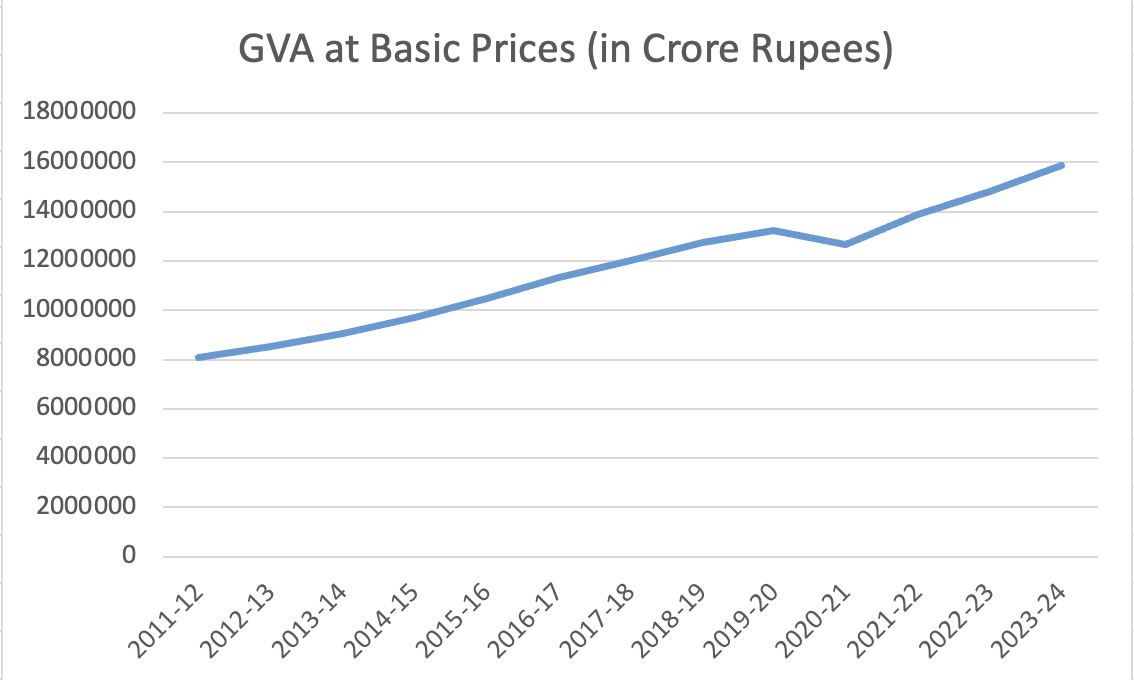
\includegraphics[width=\textwidth]{Q1/1.png}

\end{minipage}
\hfill
\begin{minipage}{0.45\textwidth}
    \centering
    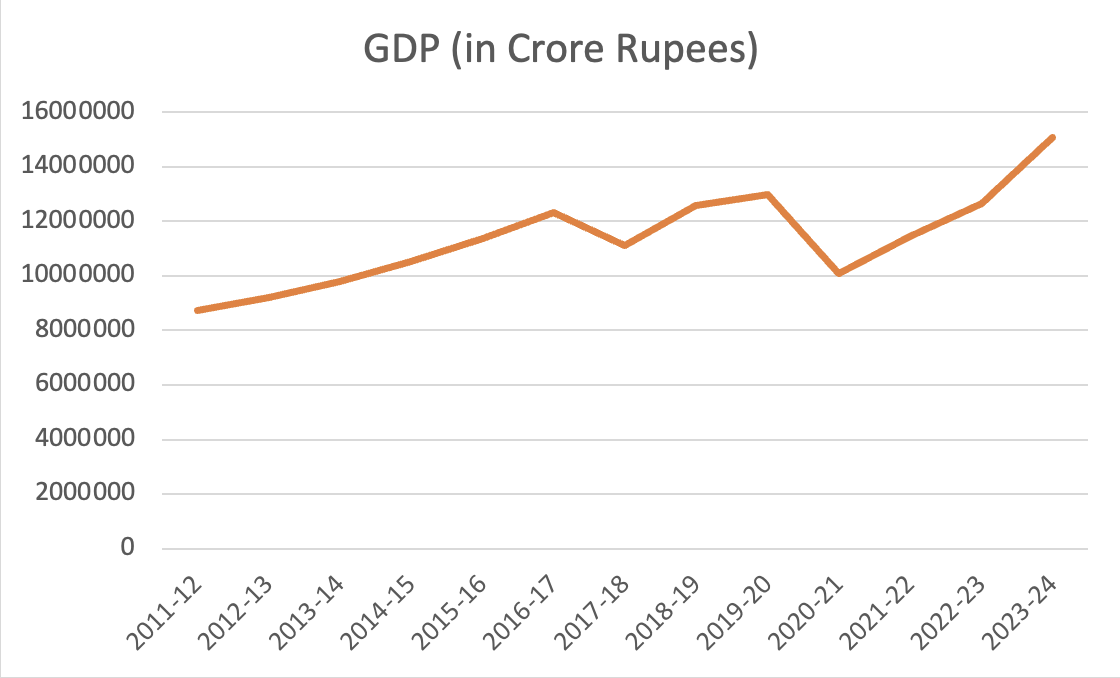
\includegraphics[width=\textwidth]{Q1/2.png}
 
\end{minipage}

\vspace{10pt} % Adds vertical space between rows

\begin{minipage}{0.45\textwidth}
    \centering
    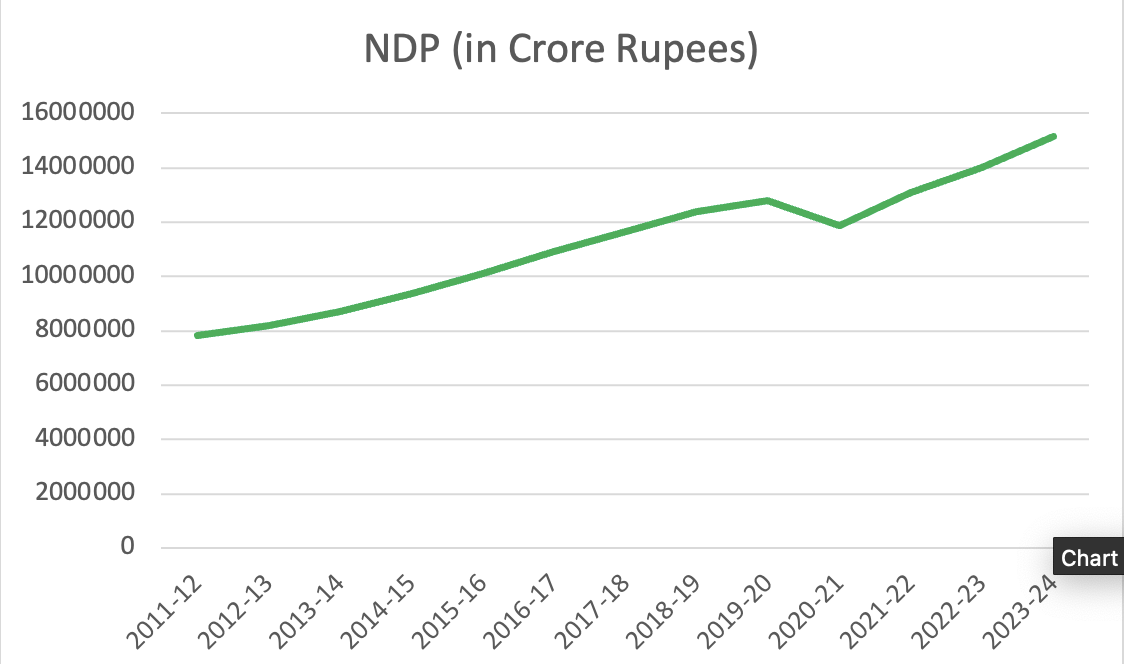
\includegraphics[width=\textwidth]{Q1/3.png}
  
\end{minipage}
\hfill
\begin{minipage}{0.45\textwidth}
    \centering
    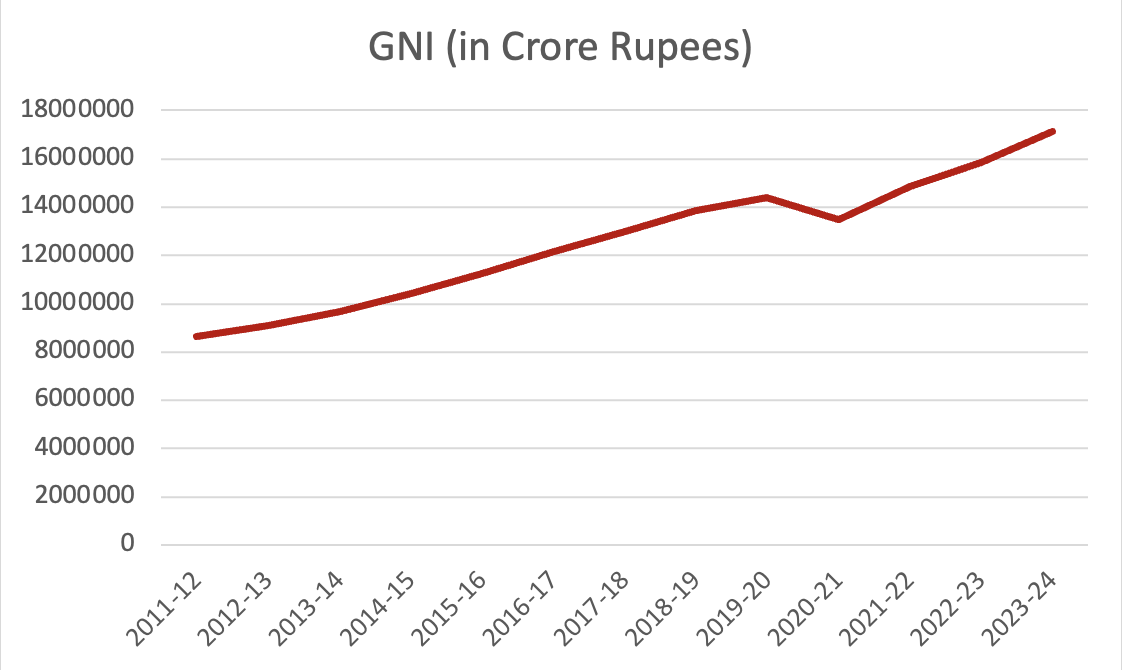
\includegraphics[width=\textwidth]{Q1/4.png}
   
\end{minipage}
\begin{center}
\centering
    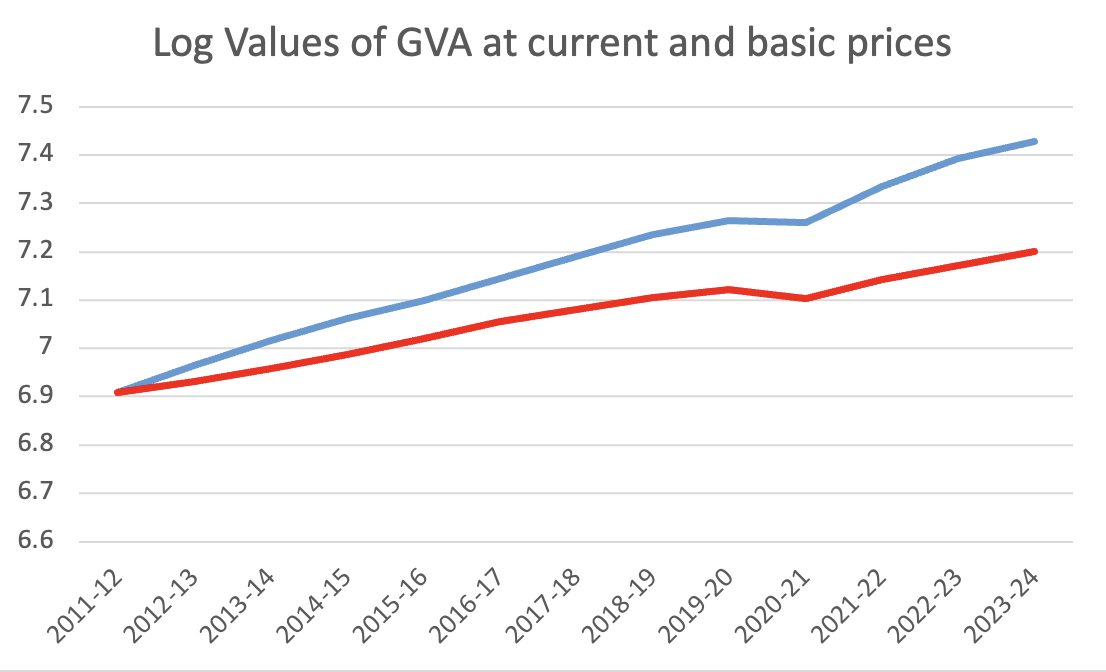
\includegraphics[width=0.45\textwidth]{Q1/5.png}
   
    
\end{center}



\\

\begin{table}[h!]
\centering
\caption{GDP, GVA, and GNI Trends in India (in Crore Rupees)}
\resizebox{\textwidth}{!}{ % Resizes the table to fit within text width
\begin{tabular}{|l|c|c|c|c|c|c|c|c|c|c|c|c|c|}
\hline
\textbf{Item/Year} & \textbf{2011-12} & \textbf{2012-13} & \textbf{2013-14} & \textbf{2014-15} & \textbf{2015-16} & \textbf{2016-17} & \textbf{2017-18} & \textbf{2018-19} & \textbf{2019-20} & \textbf{2020-21} & \textbf{2021-22} & \textbf{2022-23} & \textbf{2023-24} \\ \hline
GVA at basic prices & 8106946 & 8546275 & 9063649 & 9712133 & 10491870 & 11328285 & 12034171 & 12733798 & 13236100 & 12687345 & 13876840 & 14804901 & 15873751 \\ \hline
GDP & 8736329 & 9213017 & 9801370 & 10527674 & 11369493 & 12308193 & 11104120 & 12591160 & 12985400 & 10075250 & 11450060 & 12665280 & 15079710 \\ \hline
NDP & 7819154 & 8202356 & 8700760 & 9349029 & 10098603 & 10926667 & 11654661 & 12378459 & 12803462 & 11862110 & 13066058 & 13986798 & 15146589 \\ \hline
Gross National Income & 8659505 & 9104662 & 9679027 & 10402987 & 11234571 & 12163619 & 12998695 & 13840474 & 14392900 & 13493976 & 14827920 & 15831133 & 17125892 \\ \hline
GVA at current prices & 8106946 & 9202692 & 10363153 & 11504279 & 12574499 & 13965200 & 15505665 & 17175128 & 18381117 & 18210997 & 21635584 & 24659041 & 26762147 \\ \hline
log GVA current & 6.9 & 7.0 & 7.0 & 7.1 & 7.1 & 7.1 & 7.2 & 7.2 & 7.3 & 7.3 & 7.3 & 7.4 & 7.4 \\ \hline
log GVA basic & 6.9 & 6.9 & 7.0 & 7.0 & 7.0 & 7.1 & 7.1 & 7.1 & 7.1 & 7.1 & 7.1 & 7.2 & 7.2 \\ \hline
\end{tabular}
}

\end{table}

\subsection{Note}
\textit{
\begin{enumerate}
    \item Data for 2023-24 are Provisional Estimates.
    \item Data for 2022-23 are First Revised Estimates
    \item Data for 2021-22 are Second Revised Estimates
    \item Data for 2020-21 \& before are Third Revised Estimates
\end{enumerate}}








}
\clearpage


 \\   
    \thispagestyle{firststyle}


\\
\section{Sectoral Contributions to India’s GVA at Basic Prices (2011-12 Constant Prices)}

The composition of India’s Gross Value Added (GVA) at Basic Prices provides insights into the structural dynamics of the economy. Over the years, India has shifted gradually toward a service-driven economy, while agriculture and industry continue to play crucial roles. Here’s a sector-wise analysis:
\cite{hb20233}\cite{hb20223}\cite{hb20213}\cite{hb20203}\cite{hb20193}\cite{hb20183}

\\
\subsection{Agriculture and Allied Activities (including Forestry and Fishing)}
The Agriculture, Forestry, and Fishing sector in India has grown in absolute terms but has declined in its overall contribution to GVA. Starting at Rs. 150,194.7 crore in 2011-12, this sector reached Rs. 230,498.2 crore in 2023-24. This modest growth rate, compared to services, reflects a gradual shift in India’s economic base toward secondary and tertiary sectors. Agriculture’s declining percentage share in GVA indicates its decreasing dominance, as the economy expands and diversifies. This trend is common among emerging economies, where structural transformation pulls resources from agriculture into industry and services.

\begin{center}
    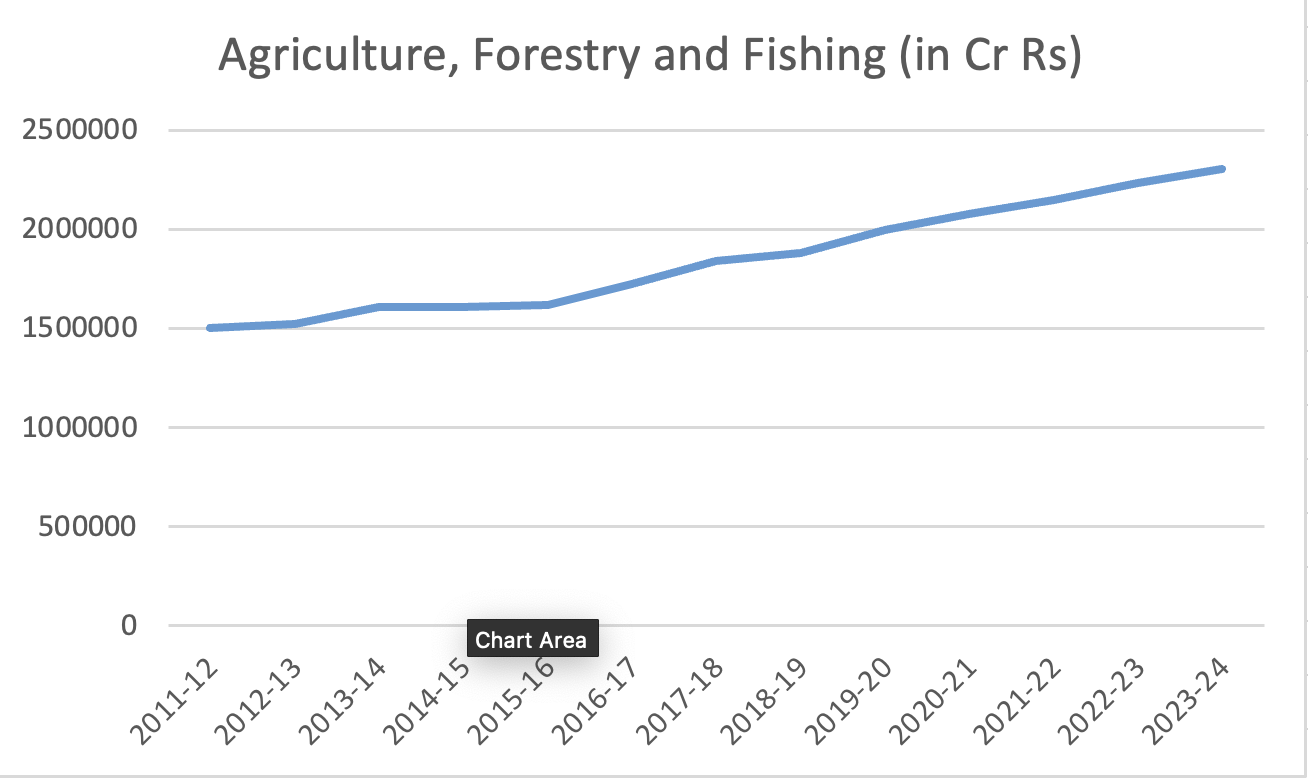
\includegraphics[width=0.7\textwidth]{Q2/1.png} 
\end{center}\\
\\
\subsection{Manufacturing}
Manufacturing remains a pillar of India’s economy, with steady growth from Rs.140,998.6 crore in 2011-12 to Rs. 275,168 crore in 2023-24. Despite its substantial growth in absolute terms, its share in GVA has shown slight declines, reflecting slower growth relative to the burgeoning services sector. India’s manufacturing sector is central to employment and exports, but its share of GDP highlights room for increased productivity and modernization. The government’s “Make in India” initiative aims to further strengthen manufacturing, which is crucial for balanced economic development.\\
\begin{center}
    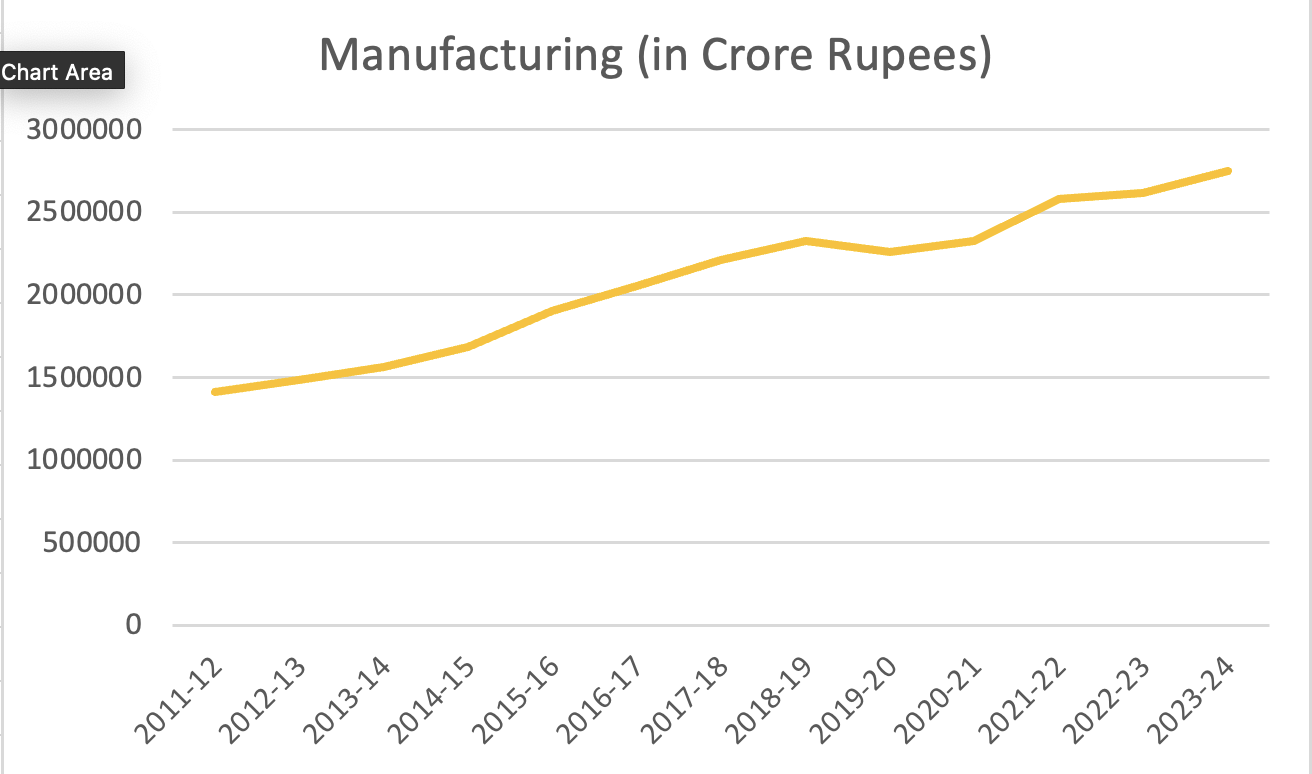
\includegraphics[width=0.7\textwidth]{Q2/2.png} 
\end{center}\\
\\
\subsection{Industry (Manufacturing, Mining \& Quarrying, Electricity, Gas, and Water Supply)}
The broader Industry sector, which includes manufacturing, mining and quarrying, and utilities (electricity, gas, and water supply), reflects the complex dynamics of the industrial economy. Starting at Rs. 185,768.9 crore in 2011-12, it grew to Rs. 346,347.8 crore in 2023-24. This sector faced periods of volatility, especially noticeable around 2020-21, likely due to external factors like global demand fluctuations and pandemic impacts. The resilience and adaptability of the industrial sector are critical to sustaining growth, creating jobs, and meeting the infrastructure needs of a growing economy.
\begin{center}
    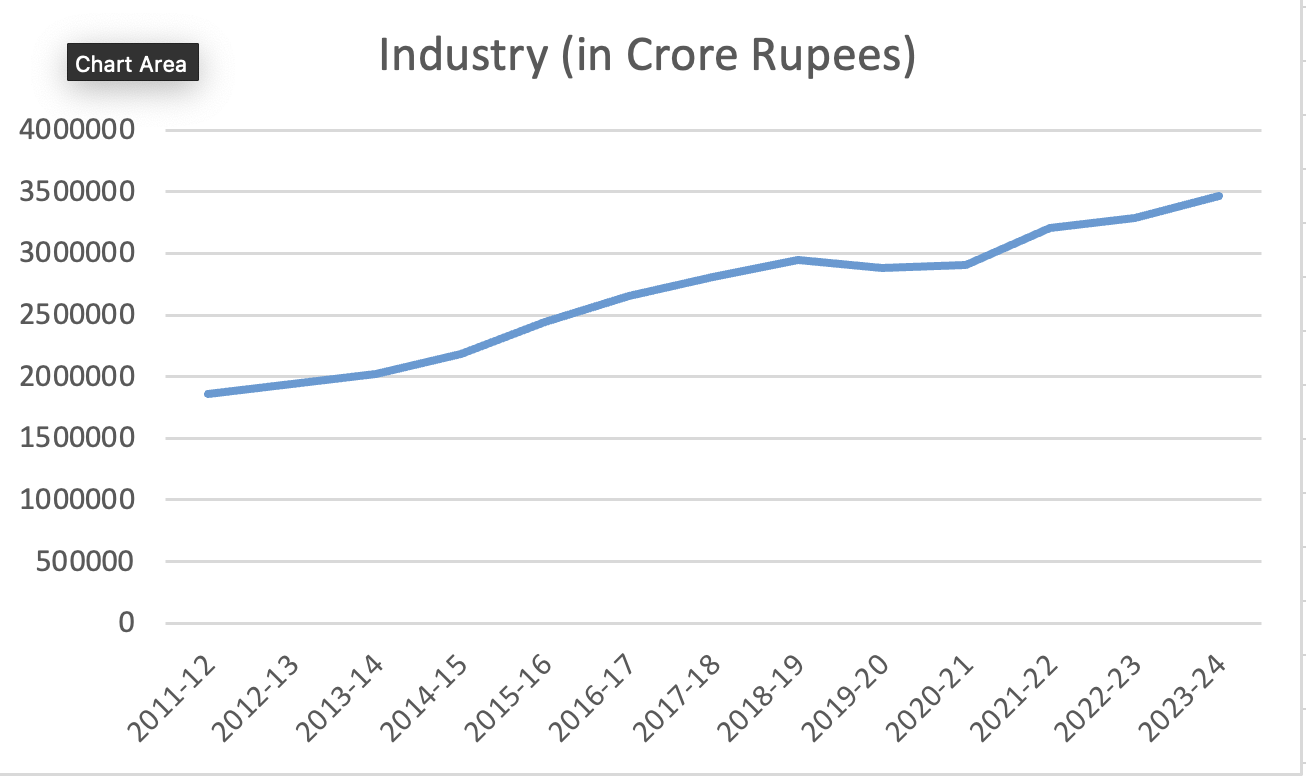
\includegraphics[width=0.7\textwidth]{Q2/3.png} 
\end{center}\\

\subsection{Construction}
The Construction sector has shown sustained growth, rising from Rs.77,733.4 crore in 2011-12 to Rs. 143,608.1 crore in 2023-24. This sector plays a dual role by providing employment and supporting infrastructure development, both vital for India’s economic advancement. The construction industry’s steady expansion aligns with India’s increased focus on infrastructure projects, urbanization, and housing development. Construction’s growth also has a ripple effect on other industries, including cement, steel, and real estate.\\

\subsection{Services}
The Services sector is by far the largest contributor to India’s GVA, expanding from Rs. 396,997.5 crore in 2011-12 to a striking Rs. 866,921 crore in 2023-24. The services sector encompasses a range of sub-sectors, including finance, IT, communication, trade, and hospitality, which have been the primary drivers of India’s economic transformation. The increasing contribution of services reflects India’s evolution into a service-led economy, fueled by advancements in IT, telecommunications, and financial services. The sector’s growth emphasizes India’s potential as a global hub for knowledge-based services, supported by a young, skilled workforce and digital innovation.
\begin{center}
    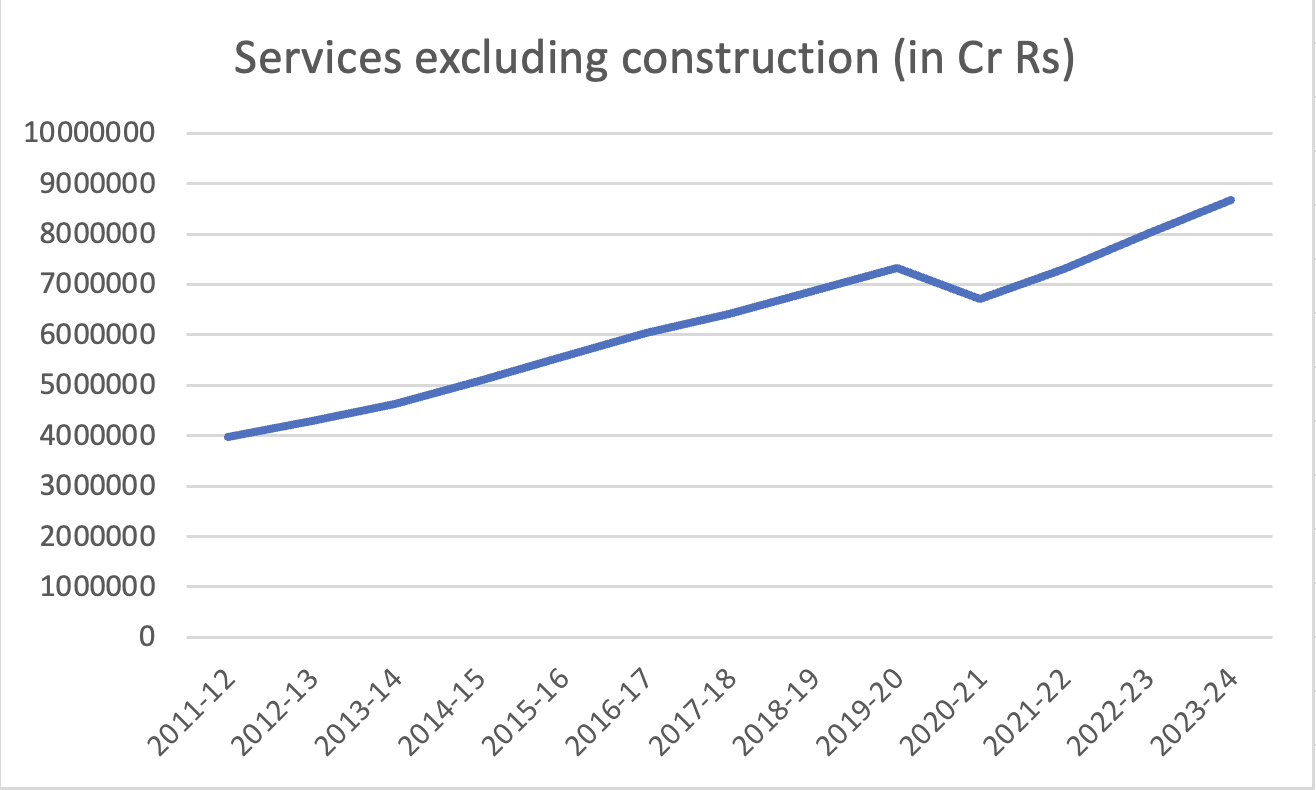
\includegraphics[width=0.7\textwidth]{Q2/4.png} 
\end{center}\\

\subsection{Components of Services}
\begin{enumerate}
    \item \textbf{Trade, Hotels, Transport, and Communication:} This segment, including trade, tourism, and transportation, grew from Rs. 141,311.6 crore in 2011-12 to Rs. 295,576.7 crore in 2023-24. The expansion highlights the growing domestic market, rising income levels, and greater connectivity across regions. Tourism and hospitality have also seen expansion, particularly as India focuses on becoming a tourism hotspot.
    
    \item \textbf{Financial, Real Estate, and Professional Services:} Increasing from Rs. 153,087.7 crore in 2011-12 to Rs. 369,164.5 crore in 2023-24, this component underscores India’s advancement in banking, real estate, insurance, and professional services. With digitalization, banking and financial services have expanded, improving financial inclusion and contributing significantly to GDP.
    
    \item \textbf{Public Administration, Defense, and Other Services:} This component grew from Rs. 102,598.2 crore in 2011-12 to Rs. 202,179.8 crore in 2023-24. These services are essential for governance, safety, and public welfare, representing a stable segment within the services sector. Growth here reflects expanded government initiatives, defense spending, and public services.
\end{enumerate}

\begin{center}
    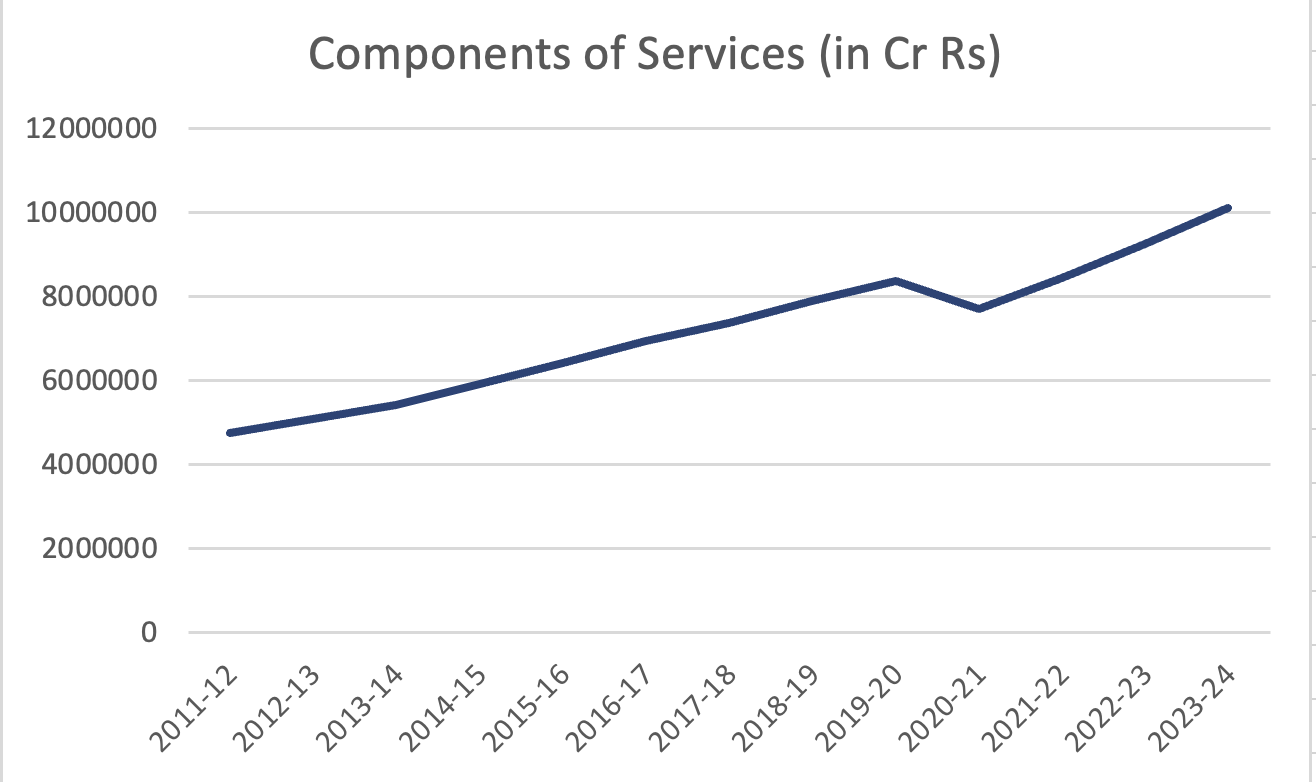
\includegraphics[width=0.7\textwidth]{Q2/5.png} 
\end{center}\\

\\
\subsection{Sectoral Shares in GDP for Agriculture, Manufacturing, and Services in India, USA, and China}
Comparing the GDP composition by sector for India, the United States, and China provides insights into the economic structures and growth trajectories of these countries.
\cite{wb}

\begin{itemize}
    \item \textbf{Agriculture, Forestry, and Fishing:}
    \begin{itemize}
        \item \textbf{India:} Agriculture’s share of GDP has been on a slight decline, from 17.2\% in 2011 to 15.97\% in 2023, which is characteristic of an economy transitioning toward industrial and service-oriented sectors. 
        \item \textbf{United States:} Agriculture contributes minimally to the U.S. GDP, steady around 1.0\%-1.3\%. 
        \item \textbf{China:} Agriculture’s share in China has steadily decreased, from 9.2\% in 2011 to 7.1\% in 2023.
    \end{itemize}

    \begin{center}
    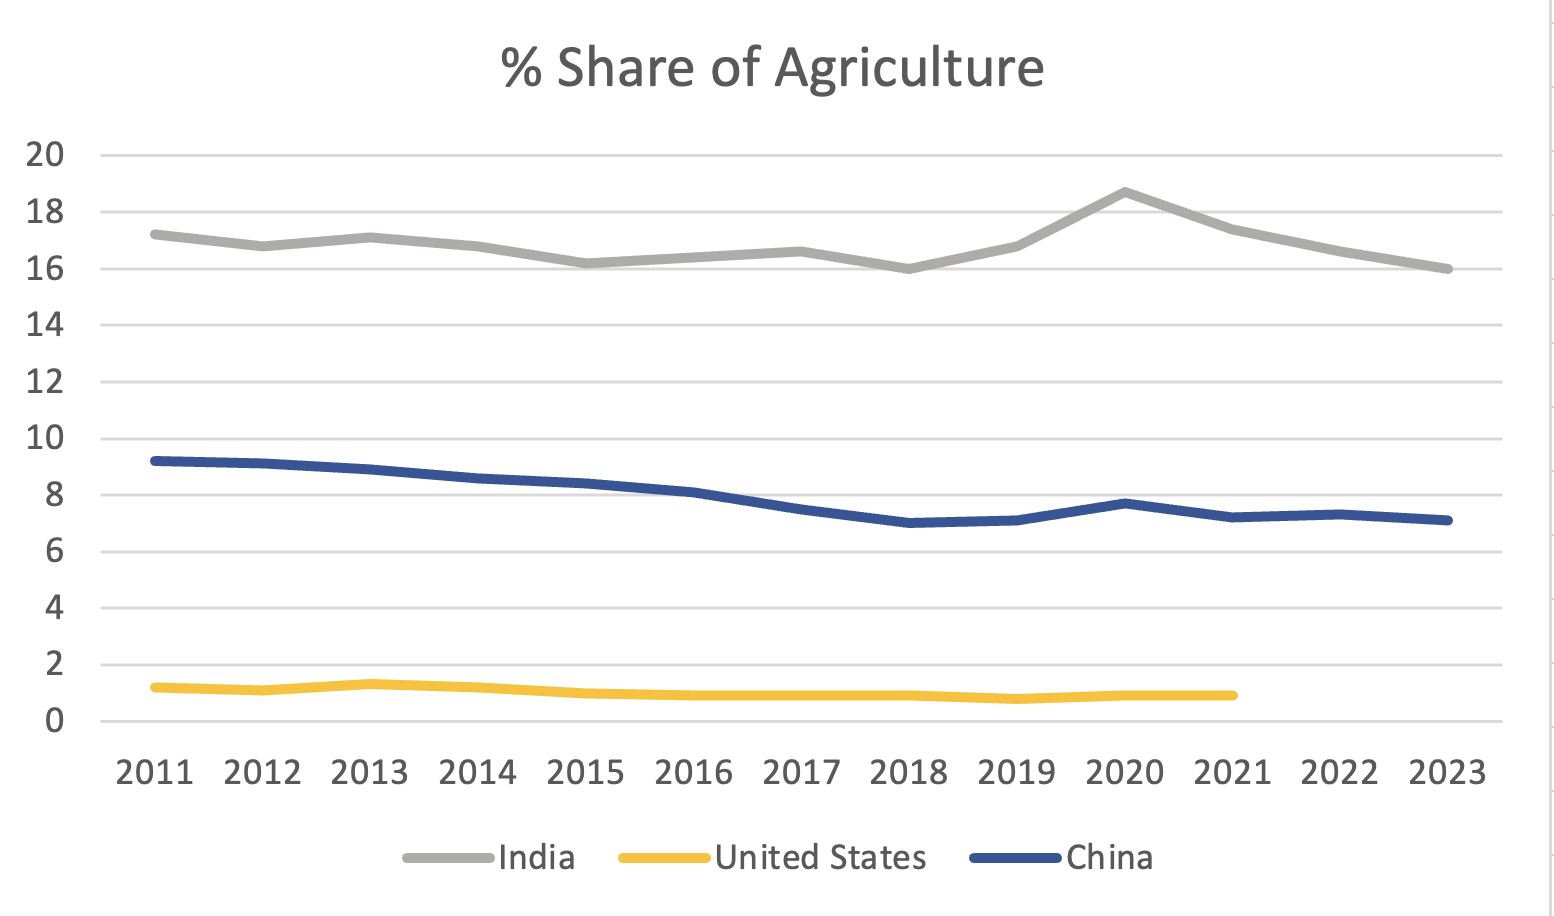
\includegraphics[width=0.7\textwidth]{Q2/6.png} 
\end{center}\\

    
    \item \textbf{Manufacturing:}
    \begin{itemize}
        \item \textbf{India:} Manufacturing’s share has decreased slightly from 16.1\% in 2011 to 12.8\% in 2023.
        \item \textbf{United States:} Manufacturing’s share has declined gradually, from 11.9\% in 2011 to 10.6\%.
        \item \textbf{China:} Manufacturing dominates China’s economy, though its share has fallen from 32.1\% in 2011 to 26.2\% in 2023.
    \end{itemize}

    \begin{center}
    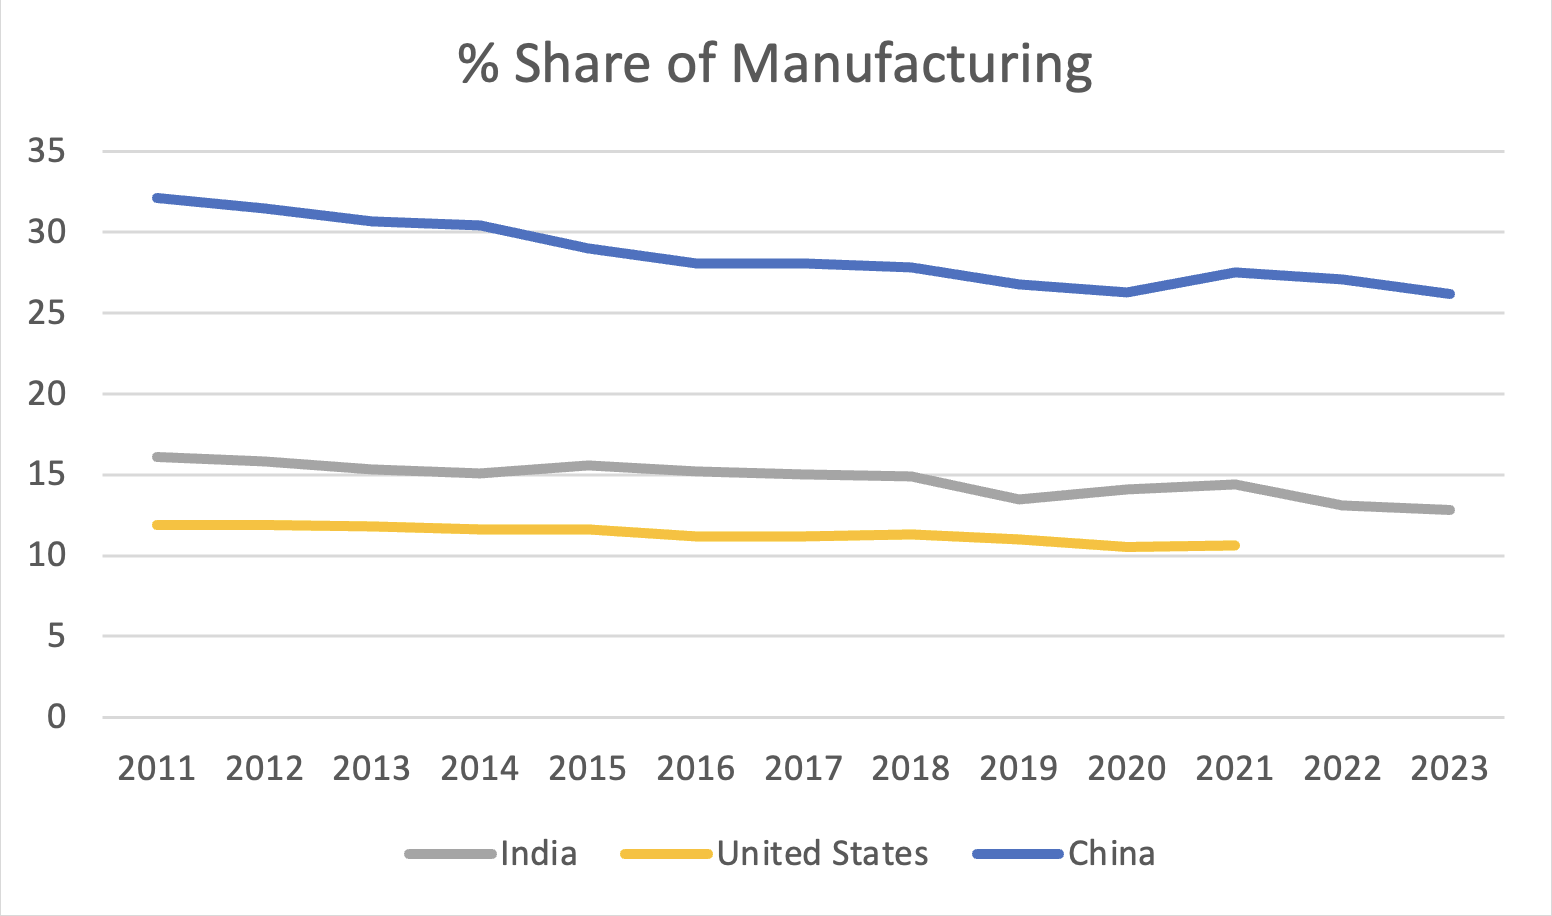
\includegraphics[width=0.7\textwidth]{Q2/7.png} 
\end{center}
\\
    
    \item \textbf{Services:}
    \begin{itemize}
        \item \textbf{India:} The services sector has expanded significantly, from 45.4\% in 2011 to 49.8\% in 2023.
        \item \textbf{United States:} Services consistently dominate the U.S. economy, contributing around 76-77\% of GDP.
        \item \textbf{China:} China’s service sector has steadily increased its share, growing from 44.3\% in 2011 to 54.6\% in 2023.
    \end{itemize}
\end{itemize}

\begin{center}
    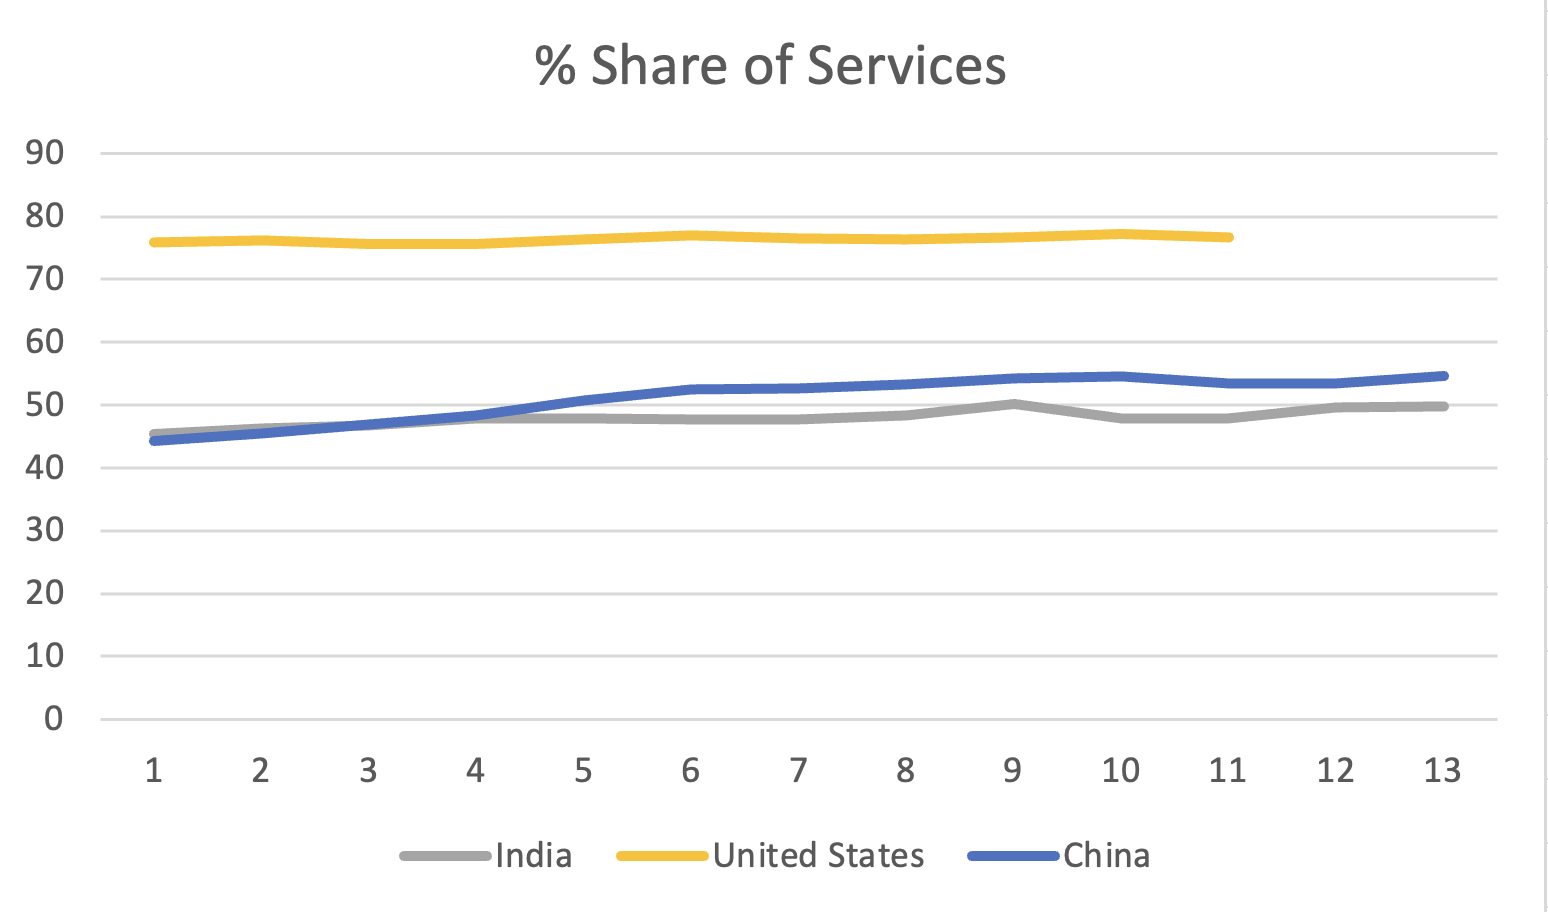
\includegraphics[width=0.7\textwidth]{Q2/8.png} 
\end{center}\\


This analysis underscores how India, the United States, and China are at different stages of economic transformation. India is experiencing a shift from agriculture to services, the U.S. is predominantly service-oriented, and China is moving from a manufacturing-led economy to one with a stronger service sector. 


\clearpage

\section{Report on GDP Composition of Selected Countries (2000–2022)}
\subsection{Abstract}
This report delves into the economic structure of China, Germany, Japan, India, and the United States by analyzing private consumption, government expenditure, and exports as shares of their GDP. Each country demonstrates unique characteristics in its economic composition, reflecting its strategic priorities, policy choices, and response to global economic trends. This analysis provides an in-depth look at these components, highlighting both short-term shifts and long-term trends across the years.\\

\cite{wb}
\subsection{China}

\paragraph{Private Consumption (C)}
\begin{itemize}
    \item Private consumption fell from 63.6\% of GDP in 2000 to 53.4\% by 2022, reflecting a policy focus on investment-driven growth.
    \item Emphasis on industrialization and infrastructure reduced consumer demand's role.
    \item Recently, China aims to boost domestic consumption to mitigate external trade pressures.
\end{itemize}

\paragraph{Government Expenditure (G)}
\begin{itemize}
    \item Government spending has remained steady at 16-18\% of GDP.
    \item Increases during economic slowdowns (2008 crisis, COVID-19) stabilize without major GDP shifts.
\end{itemize}

\paragraph{Exports (E)}
\begin{itemize}
    \item Exports rose from 23\% in 2000, peaking at 36\% in 2006; by 2022, they declined to 20.8\%.
    \item Shift toward domestic growth while exports remain key, especially in manufacturing and tech.
\end{itemize}

\paragraph{Overall Trend}
\begin{itemize}
    \item China’s economy is shifting from exports and investment to fostering domestic demand, aiming for a balanced “dual circulation” model.
\end{itemize}

\subsection{Germany}

\paragraph{Private Consumption (C)}
\begin{itemize}
    \item Consumption is stable at 73-76\% of GDP, driven by a mature economy and strong middle class.
    \item Reflects Germany’s welfare system, providing stability in domestic demand.
\end{itemize}

\paragraph{Government Expenditure (G)}
\begin{itemize}
    \item Government spending is steady at 19-22\% of GDP, supporting social services.
    \item Recent increases respond to economic uncertainties, highlighting Germany’s social market model.
\end{itemize}

\paragraph{Exports (E)}
\begin{itemize}
    \item Exports rose from 30.8\% to 50.9\% of GDP by 2022, emphasizing Germany’s strong industrial base.
    \item Export-dependence makes Germany sensitive to global market shifts.
\end{itemize}

\paragraph{Overall Trend}
\begin{itemize}
    \item Germany’s economy relies on exports, with stable government spending and a strong consumption base, supporting resilience and global competitiveness.
\end{itemize}

\subsection{Japan}

\paragraph{Private Consumption (C)}
\begin{itemize}
    \item Consumption remains high at 72-77\% of GDP, driven by domestic demand and an aging population.
    \item Japan’s high consumption base provides economic stability but is challenged by demographic shifts.
\end{itemize}

\paragraph{Government Expenditure (G)}
\begin{itemize}
    \item Government spending rose from 17\% to 21\% of GDP to counter economic stagnation.
    \item Reflects Japan’s fiscal policies aimed at growth stimulation and addressing low growth.
\end{itemize}

\paragraph{Exports (E)}
\begin{itemize}
    \item Exports increased from 10.5\% to 21.5\% of GDP, though slower than other export-oriented economies.
    \item Faces challenges from competition and aging workforce, with a diversified export portfolio.
\end{itemize}

\paragraph{Overall Trend}
\begin{itemize}
    \item Japan’s economy is consumption-driven, with stable government spending and gradual export growth, though demographic issues limit long-term growth.
\end{itemize}

\subsection{India}

\paragraph{Private Consumption (C)}
\begin{itemize}
    \item Consumption exceeds 70\% of GDP, driven by strong domestic demand and a growing middle class.
    \item Provides resilience against global economic shifts.
\end{itemize}

\paragraph{Government Expenditure (G)}
\begin{itemize}
    \item Limited government role at 10-12\% of GDP, with recent increases focused on infrastructure and social welfare.
\end{itemize}

\paragraph{Exports (E)}
\begin{itemize}
    \item Exports grew from 13\% to 23\% of GDP by 2022, with a diverse export portfolio including IT and pharmaceuticals.
    \item Trade initiatives aim to boost exports amid challenges.
\end{itemize}

\paragraph{Overall Trend}
\begin{itemize}
    \item India’s consumption-driven economy benefits from resilience, with moderate government spending and growing exports.
\end{itemize}

\subsection{United States}

\paragraph{Private Consumption (C)}
\begin{itemize}
    \item Private consumption remains over 68\% of GDP, reflecting a consumer-oriented economy.
\end{itemize}

\paragraph{Government Expenditure (G)}
\begin{itemize}
    \item Government spending grew from 17\% to around 23\% of GDP, driven by support during economic downturns.
\end{itemize}

\paragraph{Exports (E)}
\begin{itemize}
    \item Exports stay at 12-14\% of GDP, with a balanced approach to trade and strong domestic consumption.
\end{itemize}

\paragraph{Overall Trend}
\begin{itemize}
    \item The U.S. economy is consumer-driven with stable exports and growing government spending.
\end{itemize}

\begin{center}
    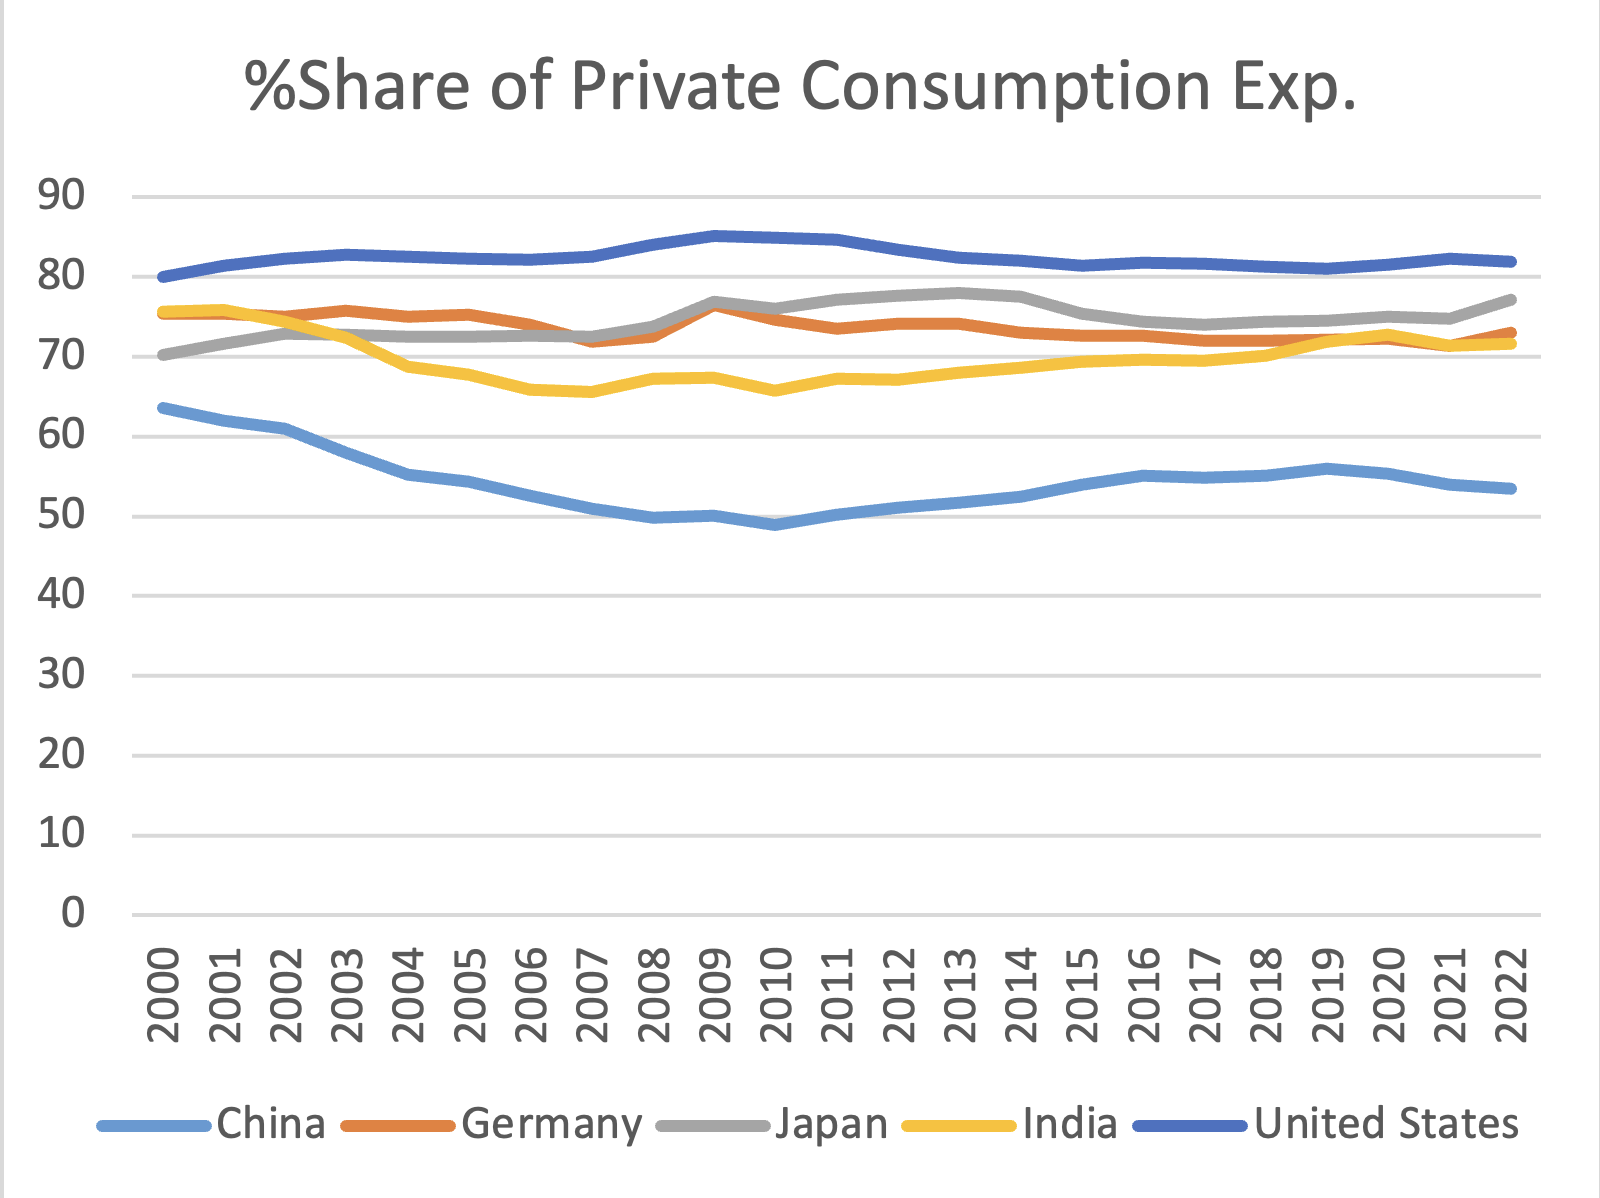
\includegraphics[width=1\textwidth]{Q3/1.png} 
\end{center}\\

\begin{center}
    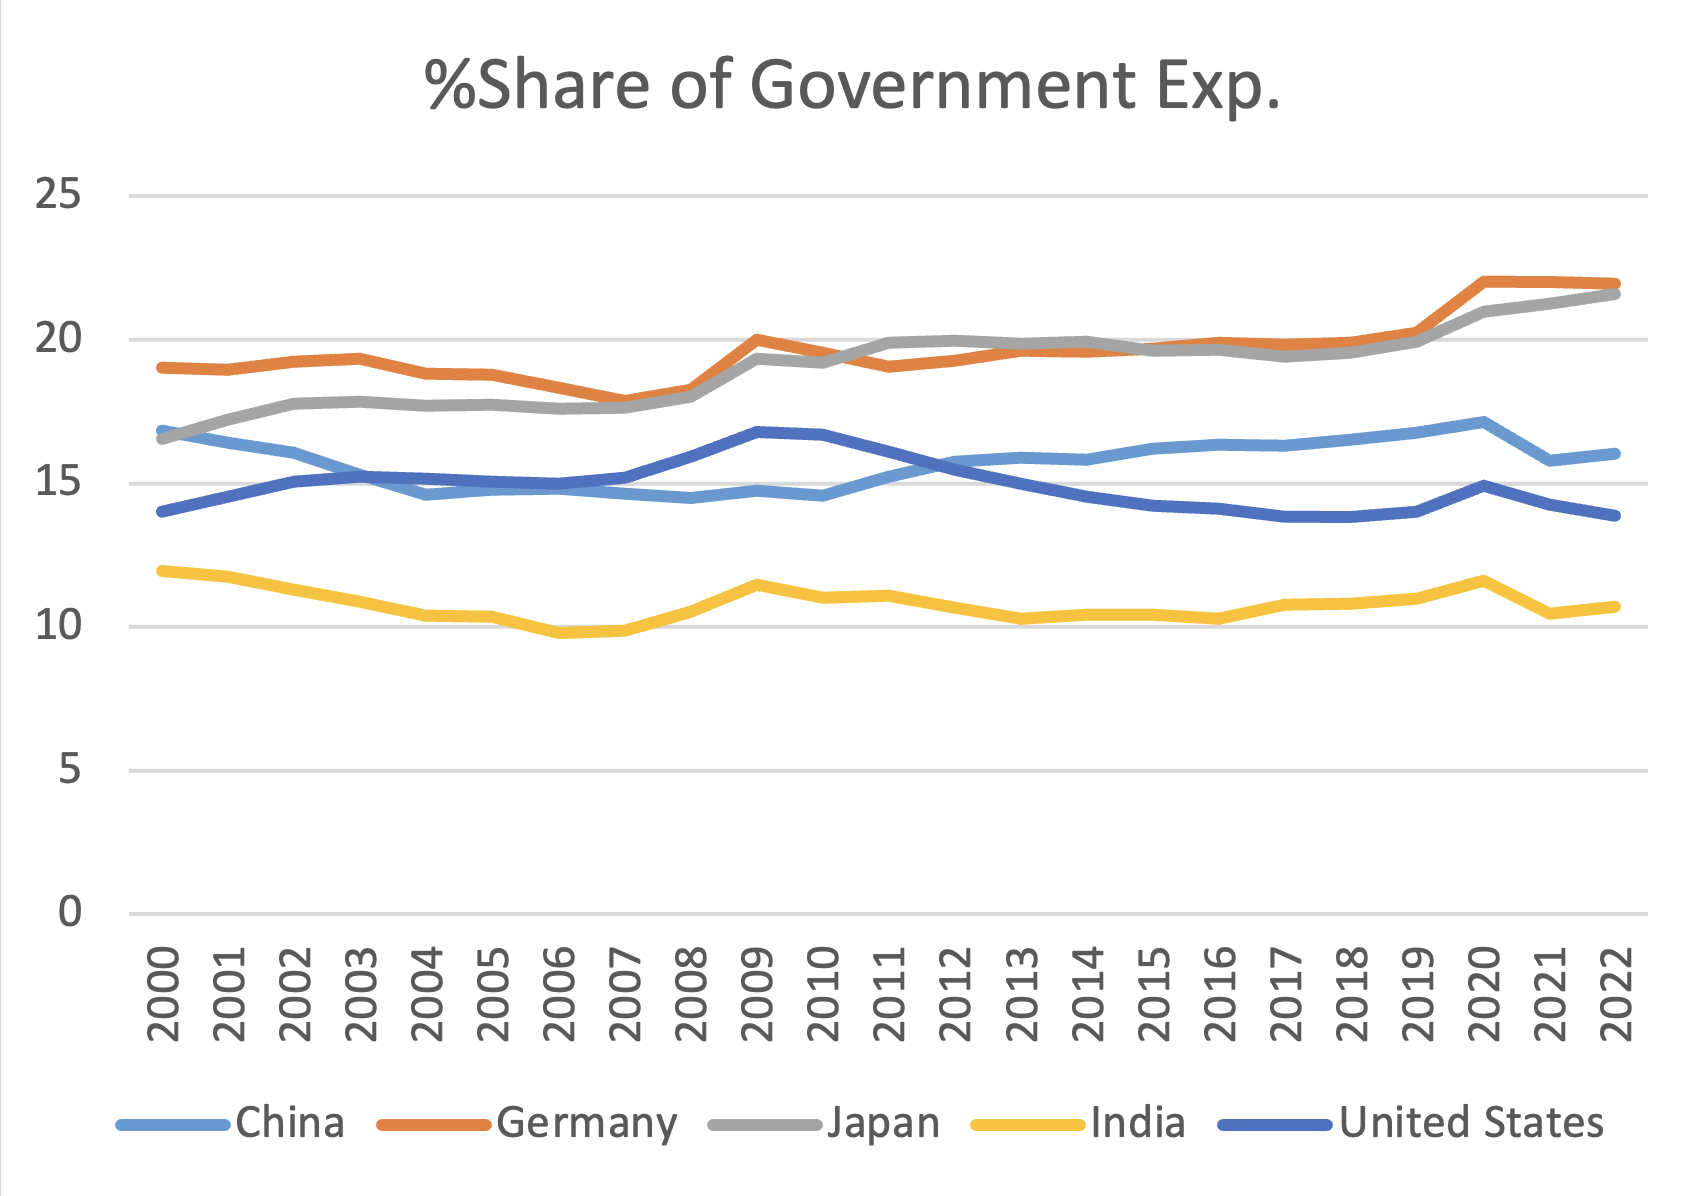
\includegraphics[width=1\textwidth]{Q3/2.png} 
\end{center}\\
\begin{center}
    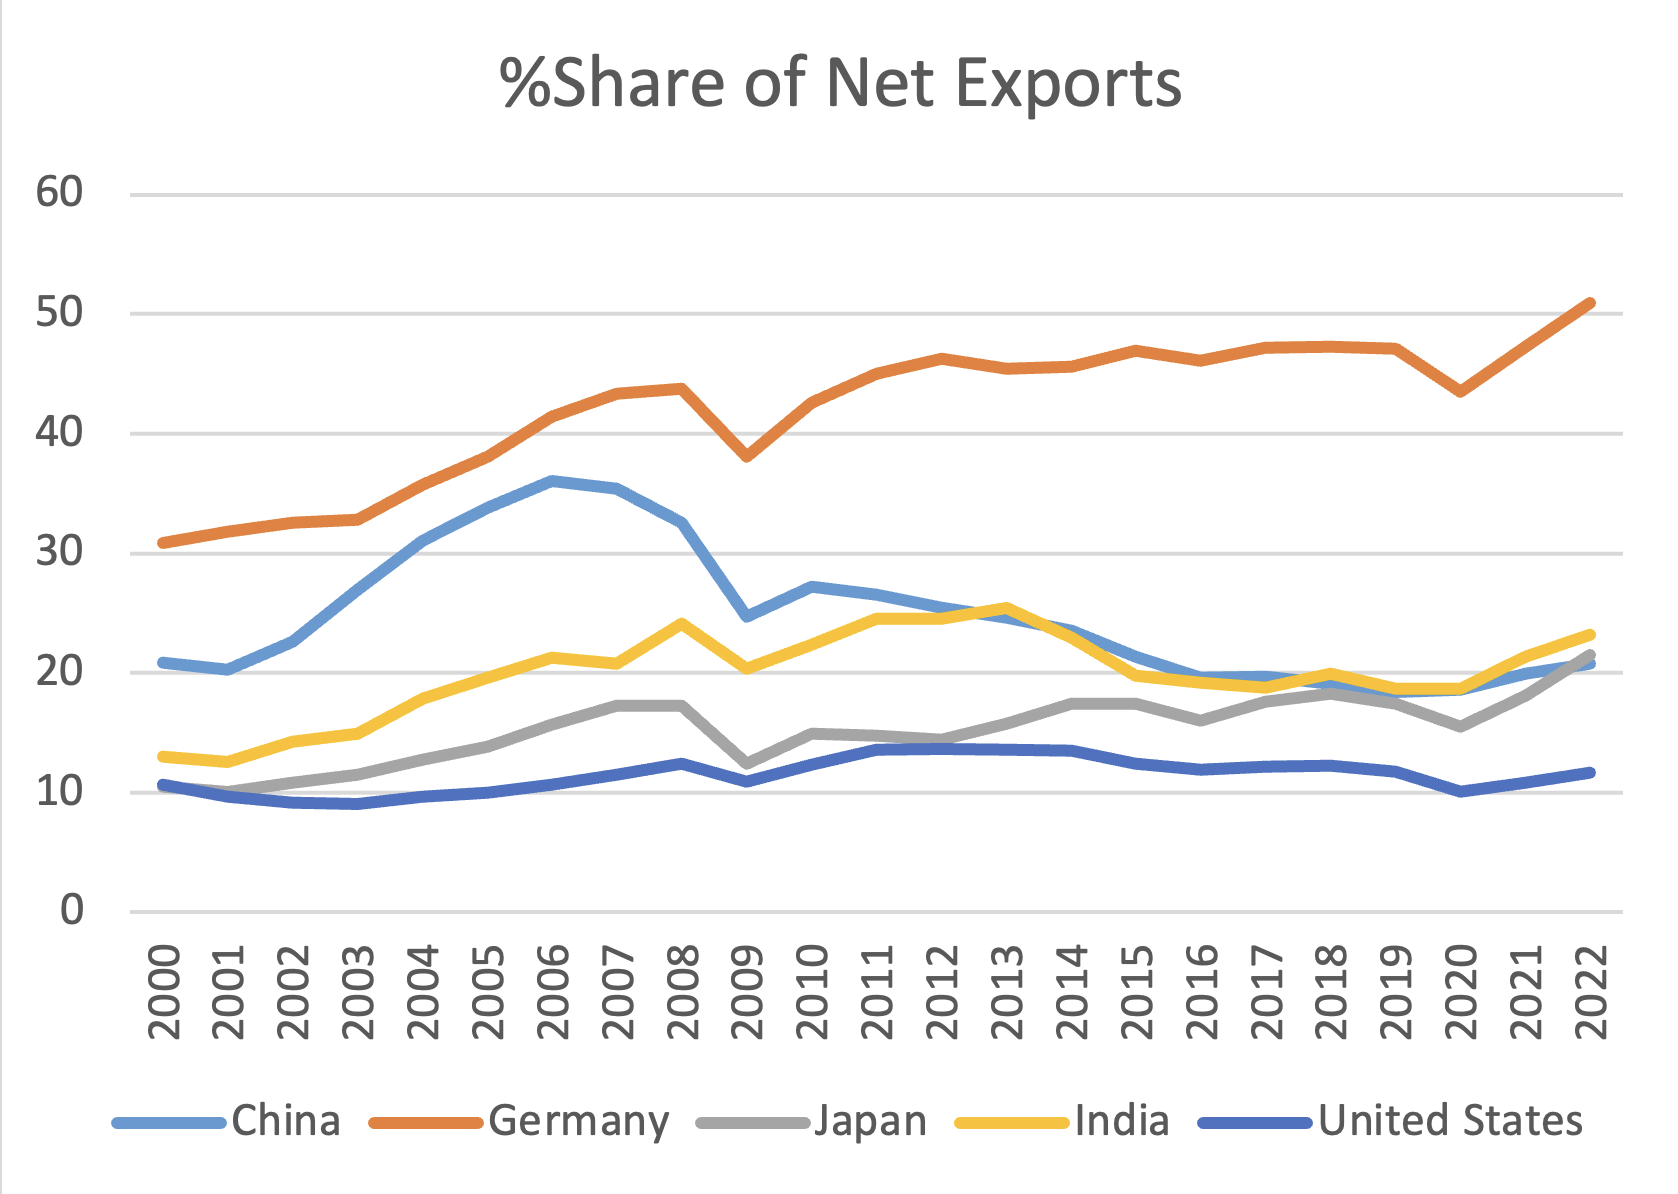
\includegraphics[width=1\textwidth]{Q3/3.png} 
\end{center}\\

\subsection{Note}
\textit{
\begin{enumerate}
    \item Data for 2023-24 are Provisional Estimates.
    \item Data for 2022-23 are First Revised Estimates
    \item Data for 2021-22 are Second Revised Estimates
    \item Data for 2020-21 \& before are Third Revised Estimates
\end{enumerate}}

\clearpage


\section{Comparative analysis of the Wholesale Price Index (WPI) and Consumer Price Index (CPI)}

\subsection{Abstract}
This part provides a comparative analysis of the Wholesale Price Index (WPI) and Consumer Price Index (CPI) inflation measures in India. We explore definitions, weights attached to components, methods of estimation, and a review of inflation trends from historical and recent perspectives.
\cite{hb2023232}\cite{hb2022232}\cite{hb2021232}\cite{hb2020232}\cite{hb2019232}\cite{hb2018232}
\subsection{Definitions}

\subsubsection{Wholesale Price Index (WPI)}
\begin{itemize}
    \item \textbf{Definition:} WPI measures the average change in prices received by producers for their output, reflecting price changes at the wholesale level before goods reach consumers.
    \item \textbf{Emphasis:} Primarily focuses on wholesale commodities, particularly industrial products over agricultural ones.
    \item \textbf{Components:} Includes primary articles, fuel, and manufacturing products. Does not account for the services sector.
\end{itemize}

\subsubsection{Consumer Price Index (CPI)}
\begin{itemize}
    \item \textbf{Definition:} CPI measures the average change in prices paid by consumers for a basket of goods and services, reflecting retail price changes.
    \item \textbf{Emphasis:} Based on consumption patterns of households, CPI includes food, housing, clothing, fuel, and miscellaneous services.
    \item \textbf{Components:} Categories like food and beverages, housing, and fuel reflect consumer behavior more closely than WPI.
\end{itemize}

\subsection{Method of Estimation}
\begin{itemize}
    \item \textbf{WPI:} Calculated based on wholesale prices, encompassing a wide variety of commodities.
    \item \textbf{CPI:} Based on retail prices of a representative basket, representing household consumption patterns.
\end{itemize}

\subsection{Calculation of Inflation Rates}
The annual inflation rate is calculated as:
\[
\text{Inflation Rate} = \frac{\text{CPI}_{x+1} - \text{CPI}_{x}}{\text{CPI}_{x}} \times 100
\]
where $\text{CPI}_{x+1}$ represents the current Consumer Price Index, and $\text{CPI}_{x}$ is the initial CPI.

\subsubsection{Sample Data for 2023-24 and 2024-25}
Using the provided CPI data, we calculate annual inflation rates for the latest available period. The monthly values are presented below in percent:

\begin{table}[h!]
\centering
\begin{tabular}{|c|c|c|}
    \hline
    \textbf{Month} & \textbf{2023-24 (\%)} & \textbf{2024-25 (\%)} \\
    \hline
    April   & 4.7 & 4.8 \\
    May     & 4.3 & 4.8 \\
    June    & 4.9 & 5.1 \\
    July    & 7.4 & 3.5 \\
    August  & 6.8 & -   \\
    September & 5.0 & - \\
    October & 4.9 & - \\
    November & 5.6 & - \\
    December & 5.7 & - \\
    January & 5.1 & - \\
    February & 5.1 & - \\
    March   & 4.9 & - \\
    \hline
\end{tabular}
\caption{Monthly CPI Inflation Rates (in percent) for 2023-24 and 2024-25}
\label{table:inflation_rates}
\end{table}\\
\\
\subsection{Analysis of Inflation Rate}


\begin{center}
    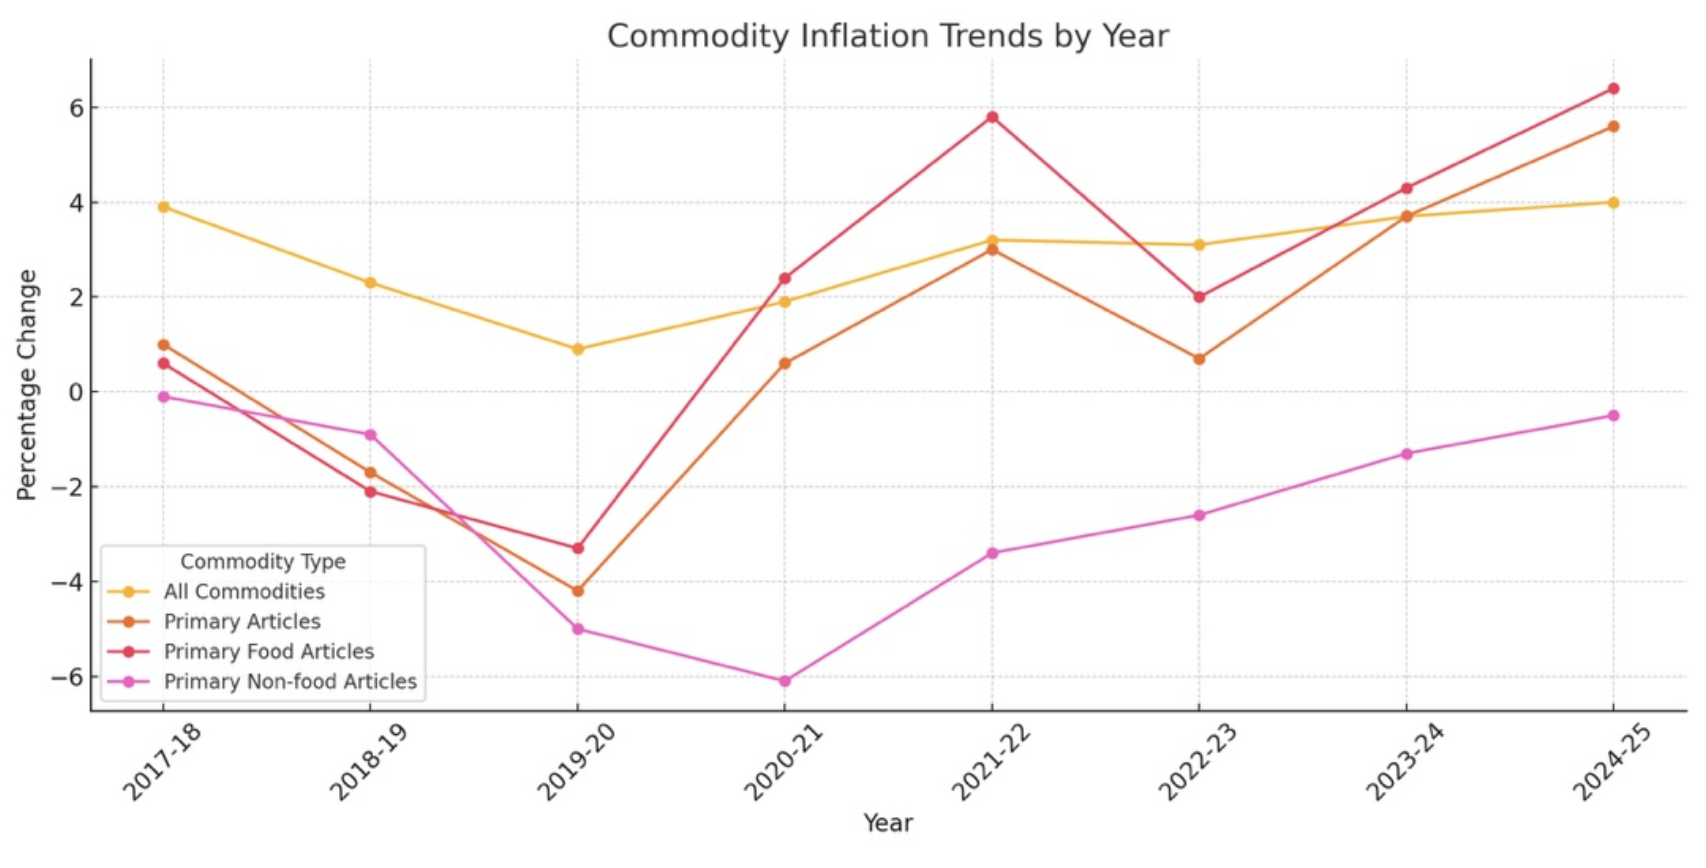
\includegraphics[width=1\textwidth]{Q5/1.png} 
\end{center}\\
\\
\begin{center}
    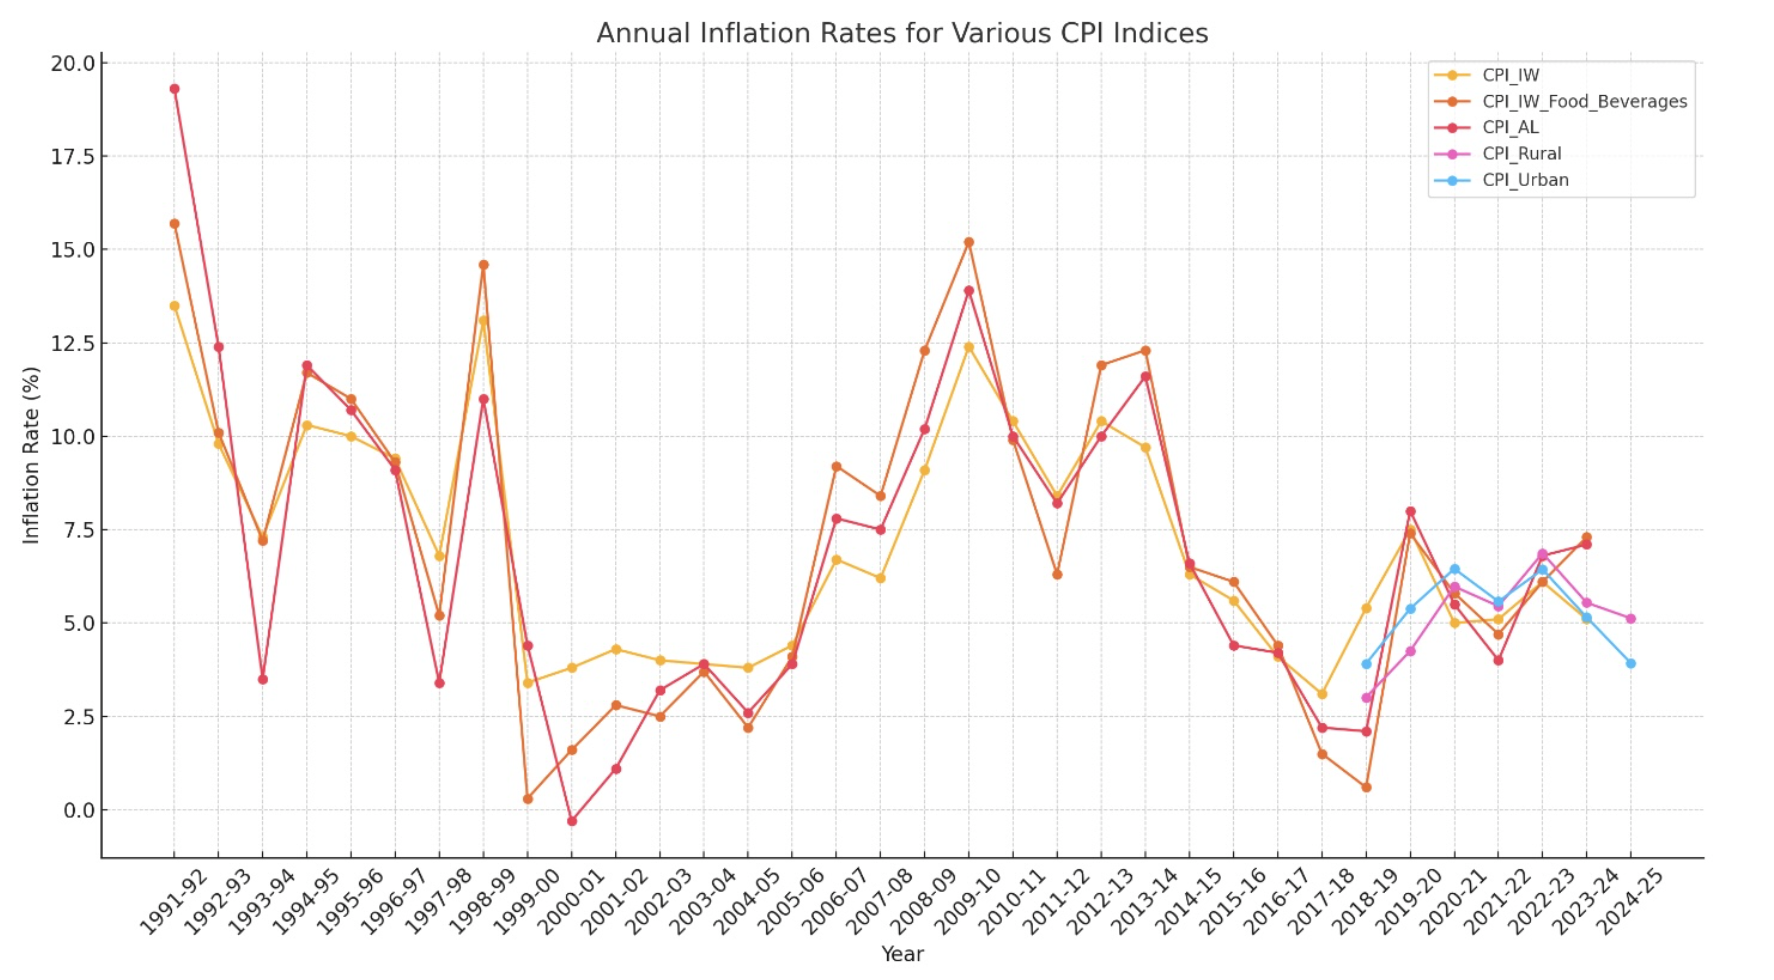
\includegraphics[width=1\textwidth]{Q5/2.png} 
\end{center}\\
\\
\begin{center}
    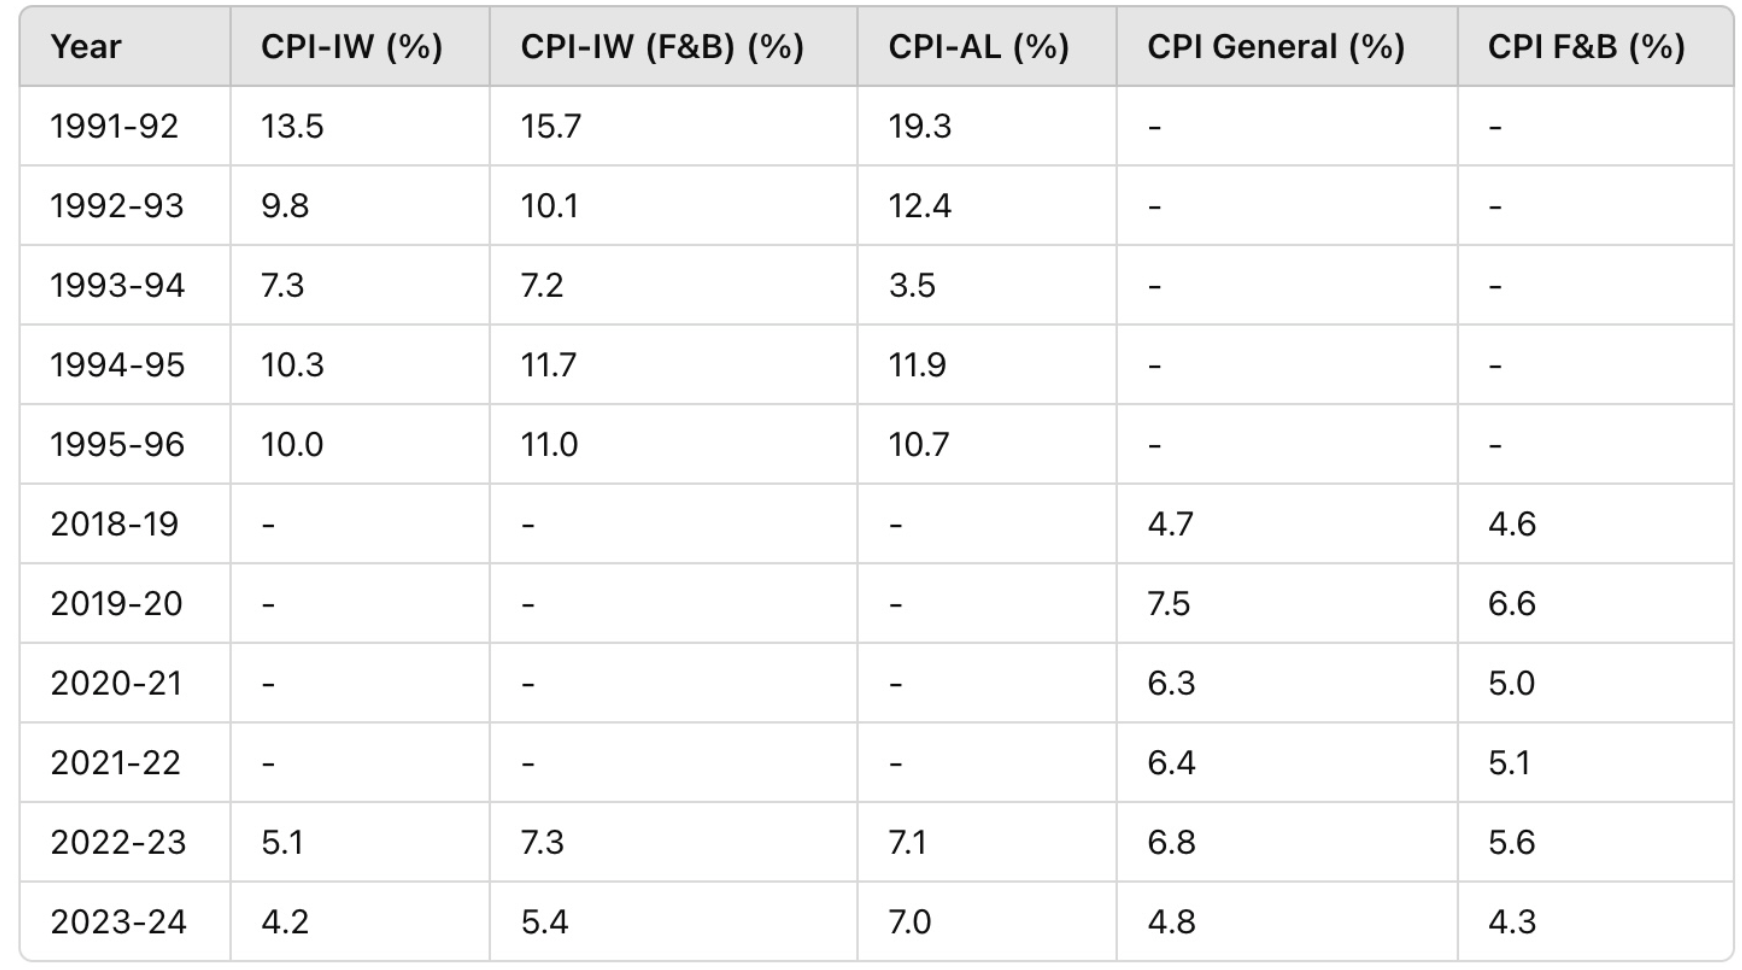
\includegraphics[width=1\textwidth]{Q5/3.png} 
\end{center}\\
\\
\begin{center}
    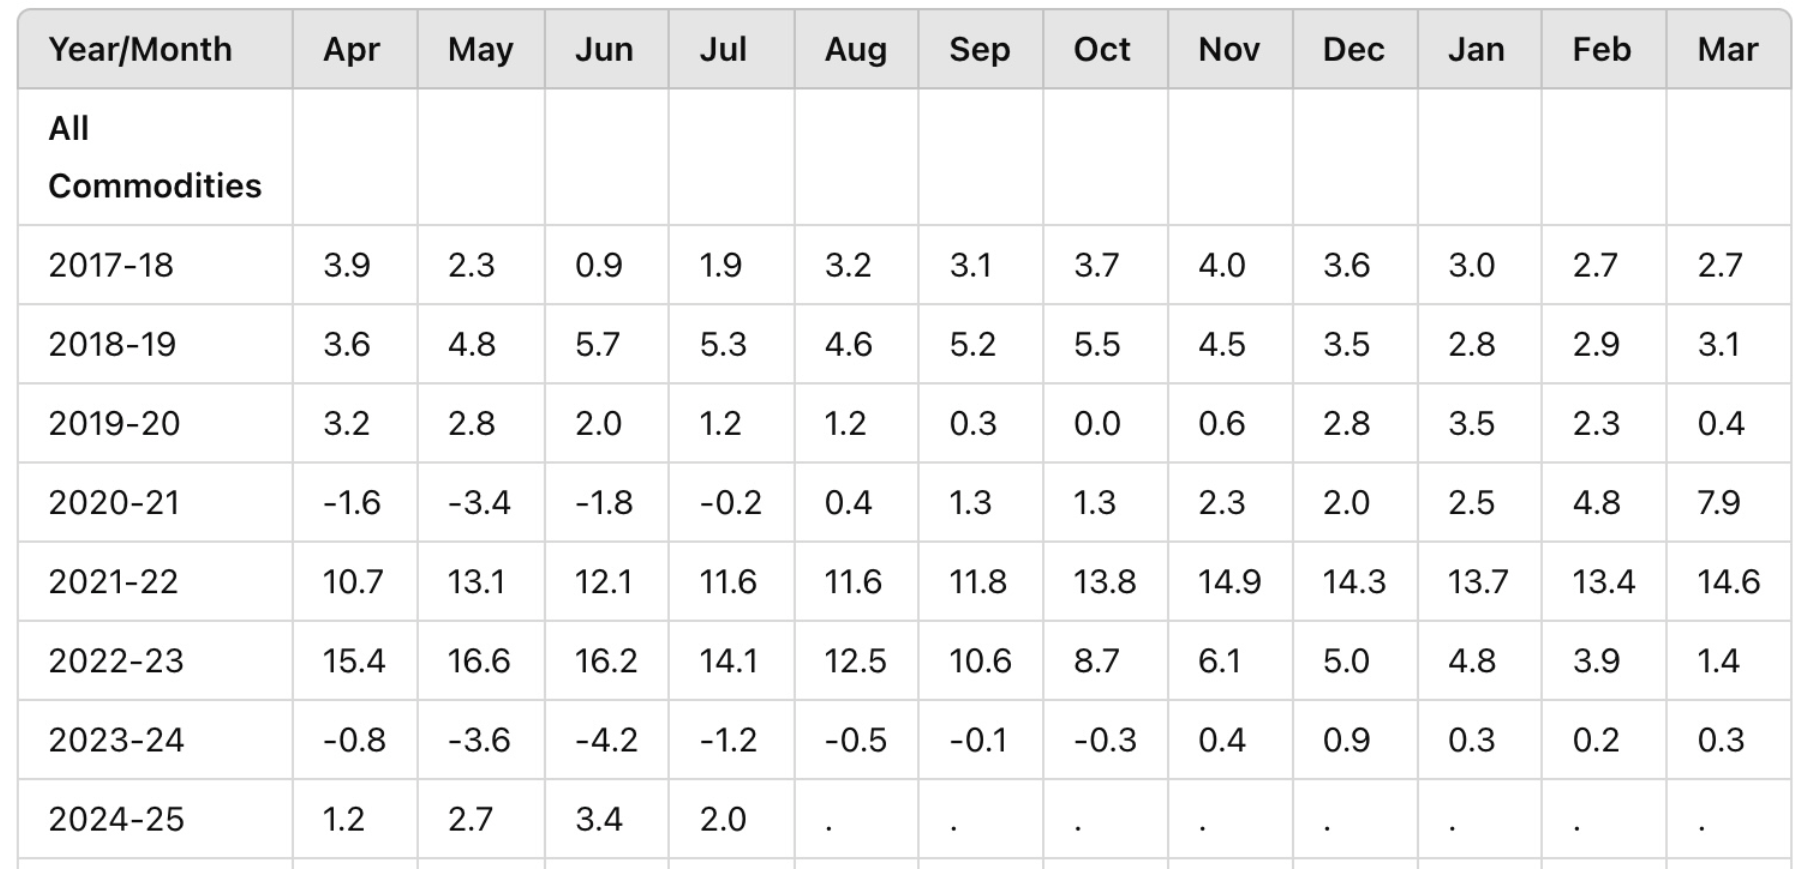
\includegraphics[width=1\textwidth]{Q5/4.png} 
\end{center}\\

\\











\subsection{General Inflation Trends and Category Insights}
\subsubsection{Period Analysis}
\begin{itemize}
    \item \textbf{2017-2020:} Low, stable inflation with brief deflation, especially in primary articles and fuel.
    \item \textbf{2020-2022:} Spike in inflation, driven by global supply chain disruptions and rising fuel costs, peaking in 2021-2022.
    \item \textbf{2023-2024:} Inflation eased with some deflation, especially in manufactured products, due to stabilization in fuel prices and supply chains.
\end{itemize}

\subsubsection{Category Insights}
\begin{itemize}
    \item \textbf{Primary Articles:} High volatility due to seasonal factors and external economic shocks, with high peaks in 2021-2022.
    \item \textbf{Fuel and Power:} Extreme fluctuations, peaking during 2021-2022, then dropping into deflation by 2023-2024.
    \item \textbf{Manufactured Products:} Stable, with temporary inflation in 2021-2022, easing back to stability in 2023.
\end{itemize}

\subsection{Combined Analysis of CPI Data for India}
\subsubsection{Overview of Inflation Trends (1991-2024)}
\begin{itemize}
    \item \textbf{1991-2024:} Initial high inflation in early 1990s, stabilization around 3-4\% by early 2000s.
    \item \textbf{2012-2020:} Moderate inflation trend, with peak inflation in 2019-20 due to food price increases.
    \item \textbf{2020-2021 (Pandemic Impact):} Supply chain disruptions caused CPI to spike, especially rural CPI.
    \item \textbf{2021-2024 (Post-Pandemic Recovery):} Gradual decline in inflation, with occasional food-related spikes.
\end{itemize}

\subsubsection{Sectoral Inflation Insights}
\begin{itemize}
    \item \textbf{Rural vs. Urban:} Rural inflation is more volatile, mainly driven by food prices, while urban inflation reflects broader economic conditions.
    \item \textbf{Food and Beverages:} Major driver of CPI increases, with higher sensitivity in rural areas.
    \item \textbf{Labor Indices:} CPI for Agricultural Laborers (AL) remains higher than Industrial Workers (IW) due to rural wage and food price dynamics.
\end{itemize}
\cite{WPI}\cite{Wpicpi}
\\
\\
This comparative analysis highlights distinct characteristics between WPI and CPI as measures of inflation, including their focus, methodology, and responses to economic shocks. Both indices offer unique insights into India's inflationary trends, relevant for policymakers and economists alike.


\subsection{Note}
\textit{
\begin{enumerate}
    \item Data for 2023-24 are Provisional Estimates.
    \item Data for 2022-23 are First Revised Estimates
    \item Data for 2021-22 are Second Revised Estimates
    \item Data for 2020-21 \& before are Third Revised Estimates
\end{enumerate}}
\clearpage







\section{Major components of Asset side of the Central Bank and Analysis}
This report examines two major components on the asset side of the Reserve Bank of India's (RBI) balance sheet: \cite{hb2023164}\cite{hb2022164}\cite{hb2021164}\cite{hb2020164}\cite{hb2019164}\cite{hb2018164}
\begin{itemize}
    \item Net RBI Credit to Government (both Central and State)
    \item Net Foreign Exchange Assets of the RBI
\end{itemize}
The data spans from April 2017 to July 2021, providing insights into how these assets have evolved over time.\\
\\
\begin{center}
    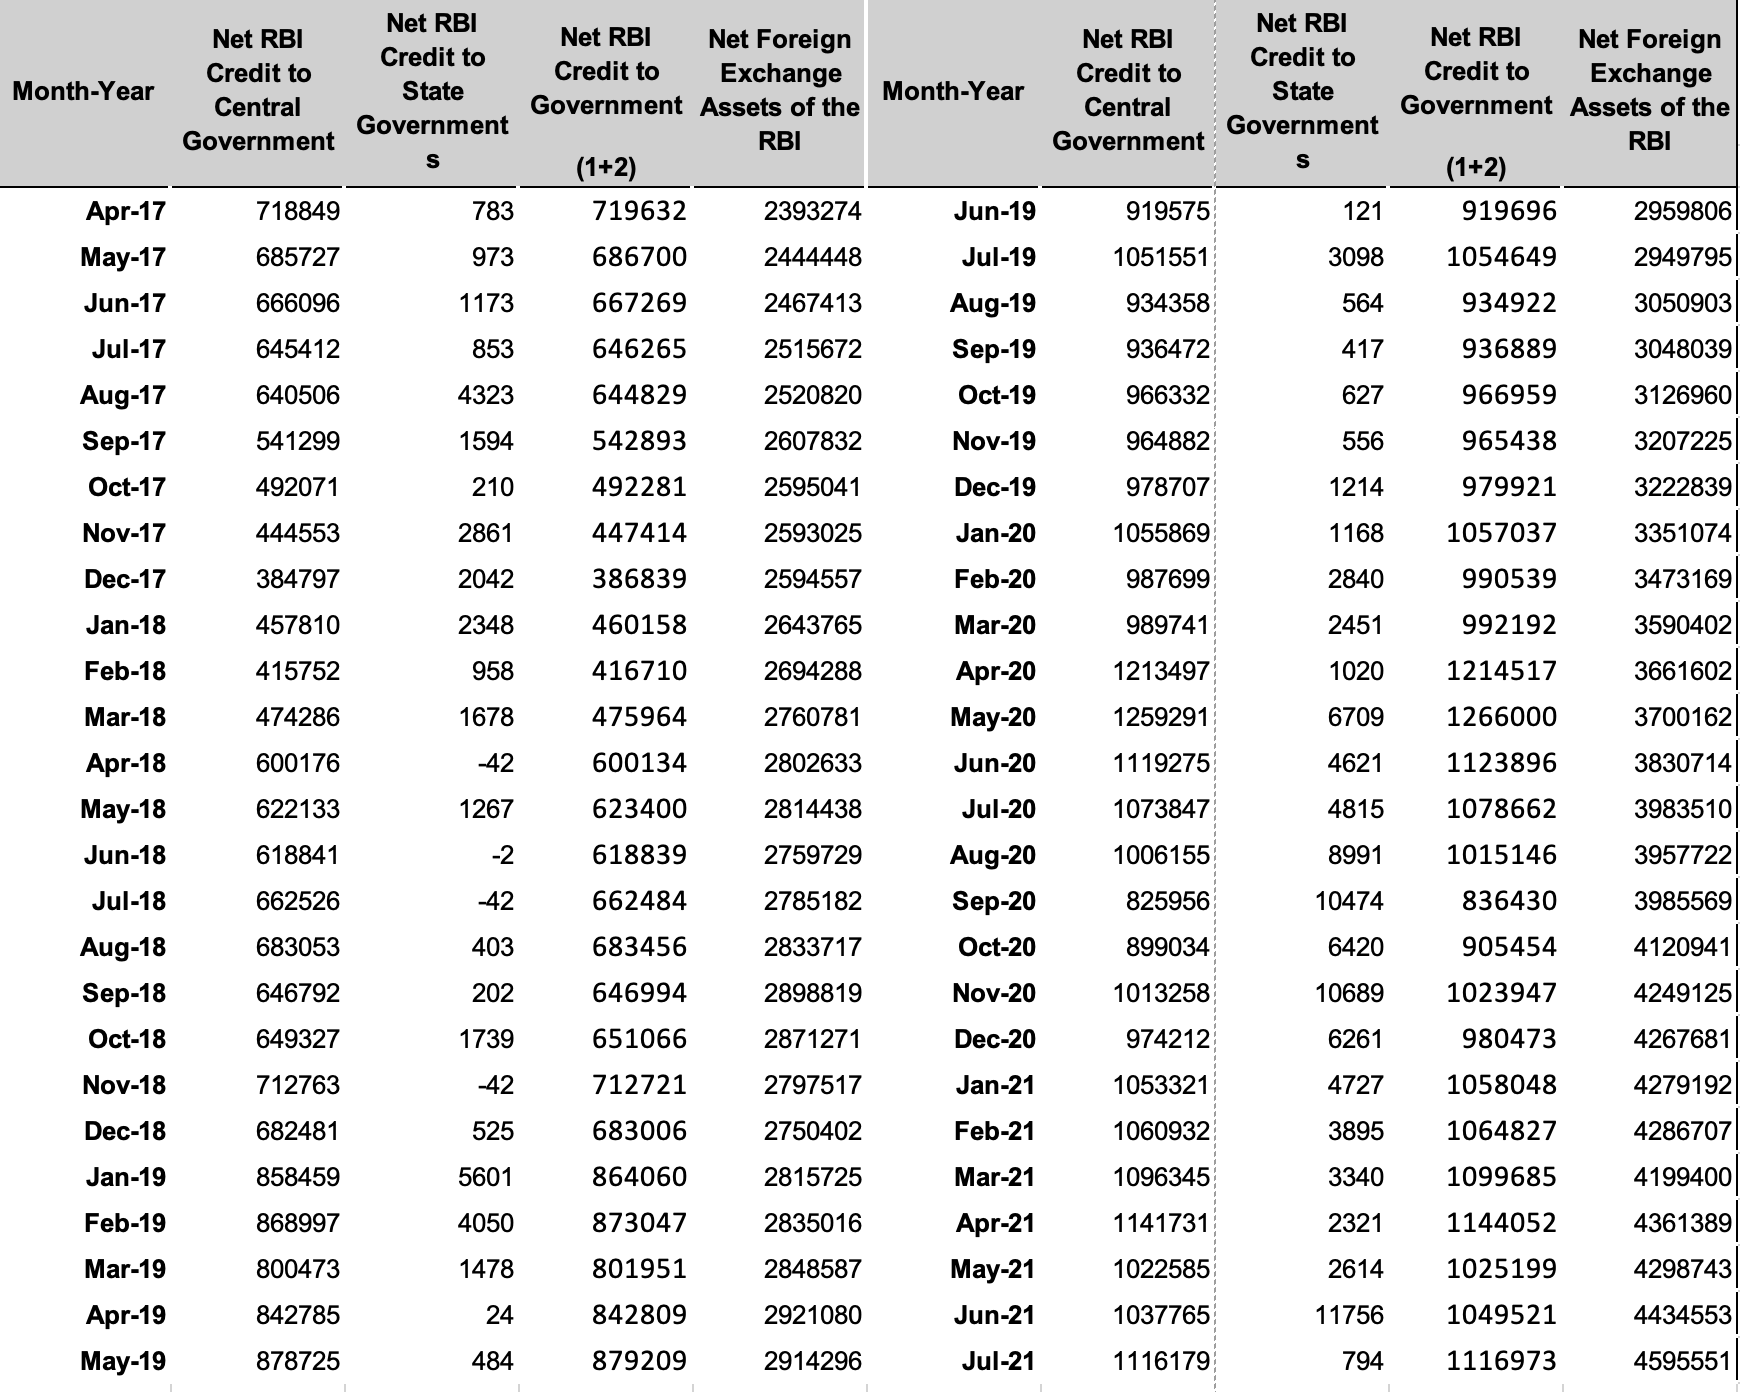
\includegraphics[width=1\textwidth]{Q7/2.png} 
\end{center}\\


\subsection{Analysis and Observations}

\begin{itemize}
    \item \textbf{Trend in Net Foreign Exchange Assets:} The chart shows a steady upward trend in the RBI's Net Foreign Exchange Assets from April 2017 to July 2021. This trend reflects India's growing foreign exchange reserves, which may be attributed to multiple factors, including trade surpluses, foreign investments, and RBI's interventions in the foreign exchange market to stabilize the rupee. Increased FX reserves bolster the country’s ability to handle economic shocks and currency volatility.
    \item \textbf{Stability in Net RBI Credit to Government:} The RBI’s credit to the government remains remarkably stable, with only minor fluctuations. However, there is a slight increase after early 2019, possibly due to the central and state governments' fiscal stimulus and financing needs. This steady trend aligns with fiscal policies where central banks provide credit to governments to support public spending, especially during economic uncertainty, providing a sense of reassurance about the fiscal policies in place.
    \item \textbf{Comparison of Trends:} The Net Foreign Exchange Assets component has grown significantly faster than RBI credit to the government. This could indicate a stronger focus on foreign reserve accumulation over domestic credit to the government, potentially aiming to strengthen macroeconomic stability and mitigate currency risk.
\end{itemize}

\subsection{Macroeconomic Implications}
In macroeconomics, we learned that the central bank’s asset movements impact the money supply. When the RBI acquires foreign assets, it increases its liabilities through currency in circulation or deposits held by private banks, which are part of reserve money. Through the money multiplier, this process raises the total money supply, influencing economic liquidity. Conversely, selling these assets would contract the money supply.

The RBI's domestic assets consist of government bonds and advances to banks. Any increase in these assets injects money into the economy, supporting investment, spending, and growth. This mechanism shows the RBI’s role in supporting economic stability while avoiding excessive inflation.

The observed trends reflect critical concepts from our macroeconomics course, such as reserve money, money multiplier, and the balance between liquidity and inflation. The RBI controls the money supply by managing foreign and domestic assets, influencing inflation and economic growth. The increase in foreign reserves and stable government credit align with a strategy focused on maintaining monetary stability and fostering a resilient economy.\cite{balsh}
\\
\\

\begin{center}
    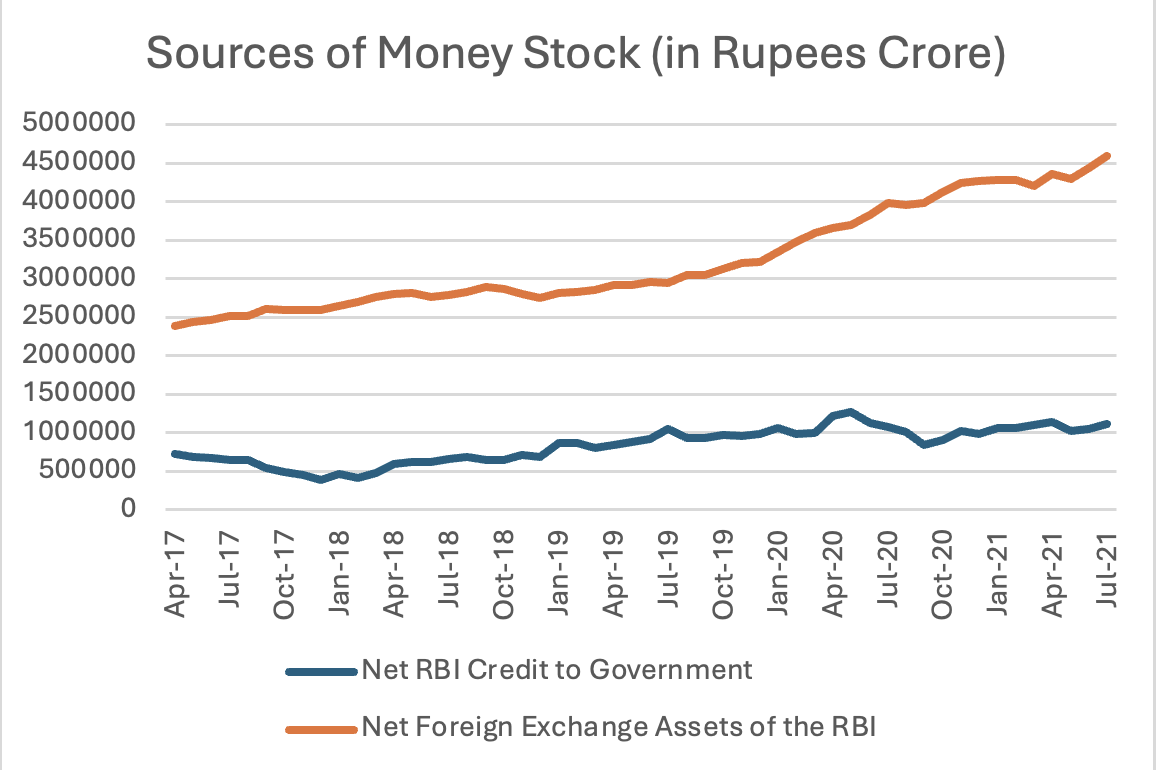
\includegraphics[width=0.7\textwidth]{Q7/Q7.png} 
\end{center}\\


\subsection{Note}
\textit{
\begin{enumerate}
    \item Data for 2023-24 are Provisional Estimates.
    \item Data for 2022-23 are First Revised Estimates
    \item Data for 2021-22 are Second Revised Estimates
    \item Data for 2020-21 \& before are Third Revised Estimates
\end{enumerate}}

\clearpage

\section{Major Components of Government's Expenditure : Analysis over the years.}

\subsection{Revenue Expenditure}
Revenue expenditure represents the government’s ongoing operational costs, covering expenses like salaries, subsidies, pensions, interest payments, and social services. This expenditure is essential for maintaining the public sector, delivering essential services, and meeting welfare commitments. Starting at Rs. 73,516 crore in 1990-91, revenue expenditure has shown a steady upward trend, reaching an estimated Rs. 37,09,401 crore by 2024-25. Key trends and drivers include:
\cite{hb202393}\cite{hb202293}\cite{hb202193}\cite{hb202093}\cite{hb201993}\cite{hb201893}

\begin{itemize}
    \item \textbf{Social Welfare Focus:} Increased spending on social services, healthcare, and education over the years has contributed significantly to the rise. Programs like the Mahatma Gandhi National Rural Employment Guarantee Act (MGNREGA), subsidies for food and fertilizers, and other welfare schemes have driven up revenue expenditure.
    \item \textbf{Interest Payments and Subsidies:} As public debt grew, interest payments became a significant expenditure. Additionally, subsidies in agriculture, food, and energy sectors have created a sustained increase in recurring expenses.
    \item \textbf{Growing Public Sector Salaries:} The government has periodically revised salaries under the Pay Commissions, which increased expenditure on wages and pensions. This reflects the government’s commitment to providing stable income to public sector employees but has also increased the rigidity of revenue spending.
\end{itemize}

\subsection{Capital Expenditure}
Capital expenditure involves spending on asset creation, infrastructure projects, and long-term investments that contribute to economic growth. It includes building roads, railways, and public enterprises. Capital expenditure was Rs. 10,874 crore in 1990-91 and rose to Rs. 2,82,773 crore in 2024-25. Notable trends include:

\begin{itemize}
    \item \textbf{Early Neglect and Recent Emphasis:} In the 1990s and early 2000s, capital expenditure remained relatively low compared to revenue spending, indicating a focus on short-term welfare over long-term infrastructure. However, since 2014, there’s been a marked increase in capital spending, highlighting the government’s shift toward investment-led growth.
    \item \textbf{Infrastructure Push:} Post-2014, initiatives like the Smart Cities Mission, Bharatmala for road connectivity, and increased railway modernization have contributed to a steady rise in capital expenditure. This increase aligns with efforts to build foundational infrastructure, improve productivity, and support private sector growth.
    \item \textbf{Strategic Asset Creation:} Investment in strategic assets, like ports, power plants, and digital infrastructure, shows the government’s intent to create a base for sustainable economic growth. However, capital expenditure still remains lower than revenue spending, which may limit its impact on the economy if not balanced effectively.
\end{itemize}

\subsection{Defence Expenditure}
Defence spending, while smaller compared to total government expenditure, is essential for national security. It covers personnel costs, weaponry, equipment, and maintenance of military infrastructure. Defence expenditure has increased from Rs. 19,652 crore in 1990-91 to Rs. 1,92,416 crore in 2024-25. Key insights include:

\begin{itemize}
    \item \textbf{Gradual Increase in Security Spending:} Defence spending has grown gradually over time, with a sharper rise in recent years. This trend aligns with heightened security concerns, both regional (border tensions) and global (military modernization).
    \item \textbf{Focus on Modernization:} The Indian government has increasingly invested in modernizing the armed forces, acquiring new equipment, and enhancing capabilities in areas like cyber defence. While still a relatively small share of total expenditure, the growing defence budget reflects the need to address strategic security risks.
    \item \textbf{Balancing Budget Constraints:} Defence expenditure increases are balanced against other welfare and development needs. This cautious approach ensures security requirements are met without excessively burdening the overall fiscal budget.
\end{itemize}

\subsection{Analysis of Trends and Observations}

\begin{enumerate}
    \item \textbf{Growth in Revenue Expenditure:} Revenue expenditure has grown continuously, often outpacing capital expenditure. This trend points to a high commitment to welfare spending but also reflects challenges in reducing recurring costs, such as salaries and subsidies. While these expenses are crucial for social welfare, they limit the government’s flexibility to shift funds to investment and infrastructure, potentially hindering long-term growth.
    \item \textbf{Rising Capital Expenditure Since 2014:} Capital expenditure, though comparatively lower, has seen a significant push in recent years, particularly after 2014. The government’s focus on infrastructure investment aims to spur economic growth, improve logistics, and make India more attractive for investment. However, the gap between revenue and capital expenditure remains considerable, indicating that operational costs and welfare schemes still dominate budget priorities.
    \item \textbf{Increased Defence Spending in Recent Years:} The rise in defence expenditure, especially in the 2020s, reflects a strategic emphasis on national security amid regional tensions and global uncertainties. This shift shows the government’s efforts to balance welfare spending with security needs. Yet, defence remains a relatively small proportion of total expenditure compared to other sectors, which may impact the speed of military modernization.
\end{enumerate}

\subsection{Broader Implications and Challenges}

\begin{itemize}
    \item \textbf{Sustainability of Revenue Expenditure:} The consistent growth in revenue expenditure, driven by salaries, subsidies, and interest payments, poses a challenge for budget sustainability. High revenue expenditure limits resources available for productive investments, potentially affecting India’s long-term fiscal health.
    \item \textbf{Balancing Capital and Revenue Expenditure:} The government faces the dual challenge of meeting immediate welfare needs while ensuring sufficient capital investment to foster economic growth. Maintaining this balance is crucial for sustainable development, as excessive revenue spending could crowd out capital expenditure.
    \item \textbf{Strategic Prioritization:} Defence and capital expenditure must be prioritized carefully to ensure both security and infrastructure goals are met without compromising fiscal stability. This balancing act is essential as India navigates economic challenges and seeks to establish itself as a strong global economy.\cite{expgov}
\end{itemize}

\\
\\
The data reflects India’s evolving fiscal priorities: balancing welfare with investment-led growth and adapting to emerging security needs. While revenue expenditure has largely dominated due to its recurring nature, the government’s increasing focus on capital expenditure and defence signals a strategic shift towards building a resilient, future-ready economy. \cite{expegov}
\\
\\
The table is annexed in the subsequent page.
\subsection{Note}
\textit{
\begin{enumerate}
    \item Data for 2023-24 are Provisional Estimates.
    \item Data for 2022-23 are First Revised Estimates
    \item Data for 2021-22 are Second Revised Estimates
    \item Data for 2020-21 \& before are Third Revised Estimates
\end{enumerate}}


\newpage  % Start on a new page
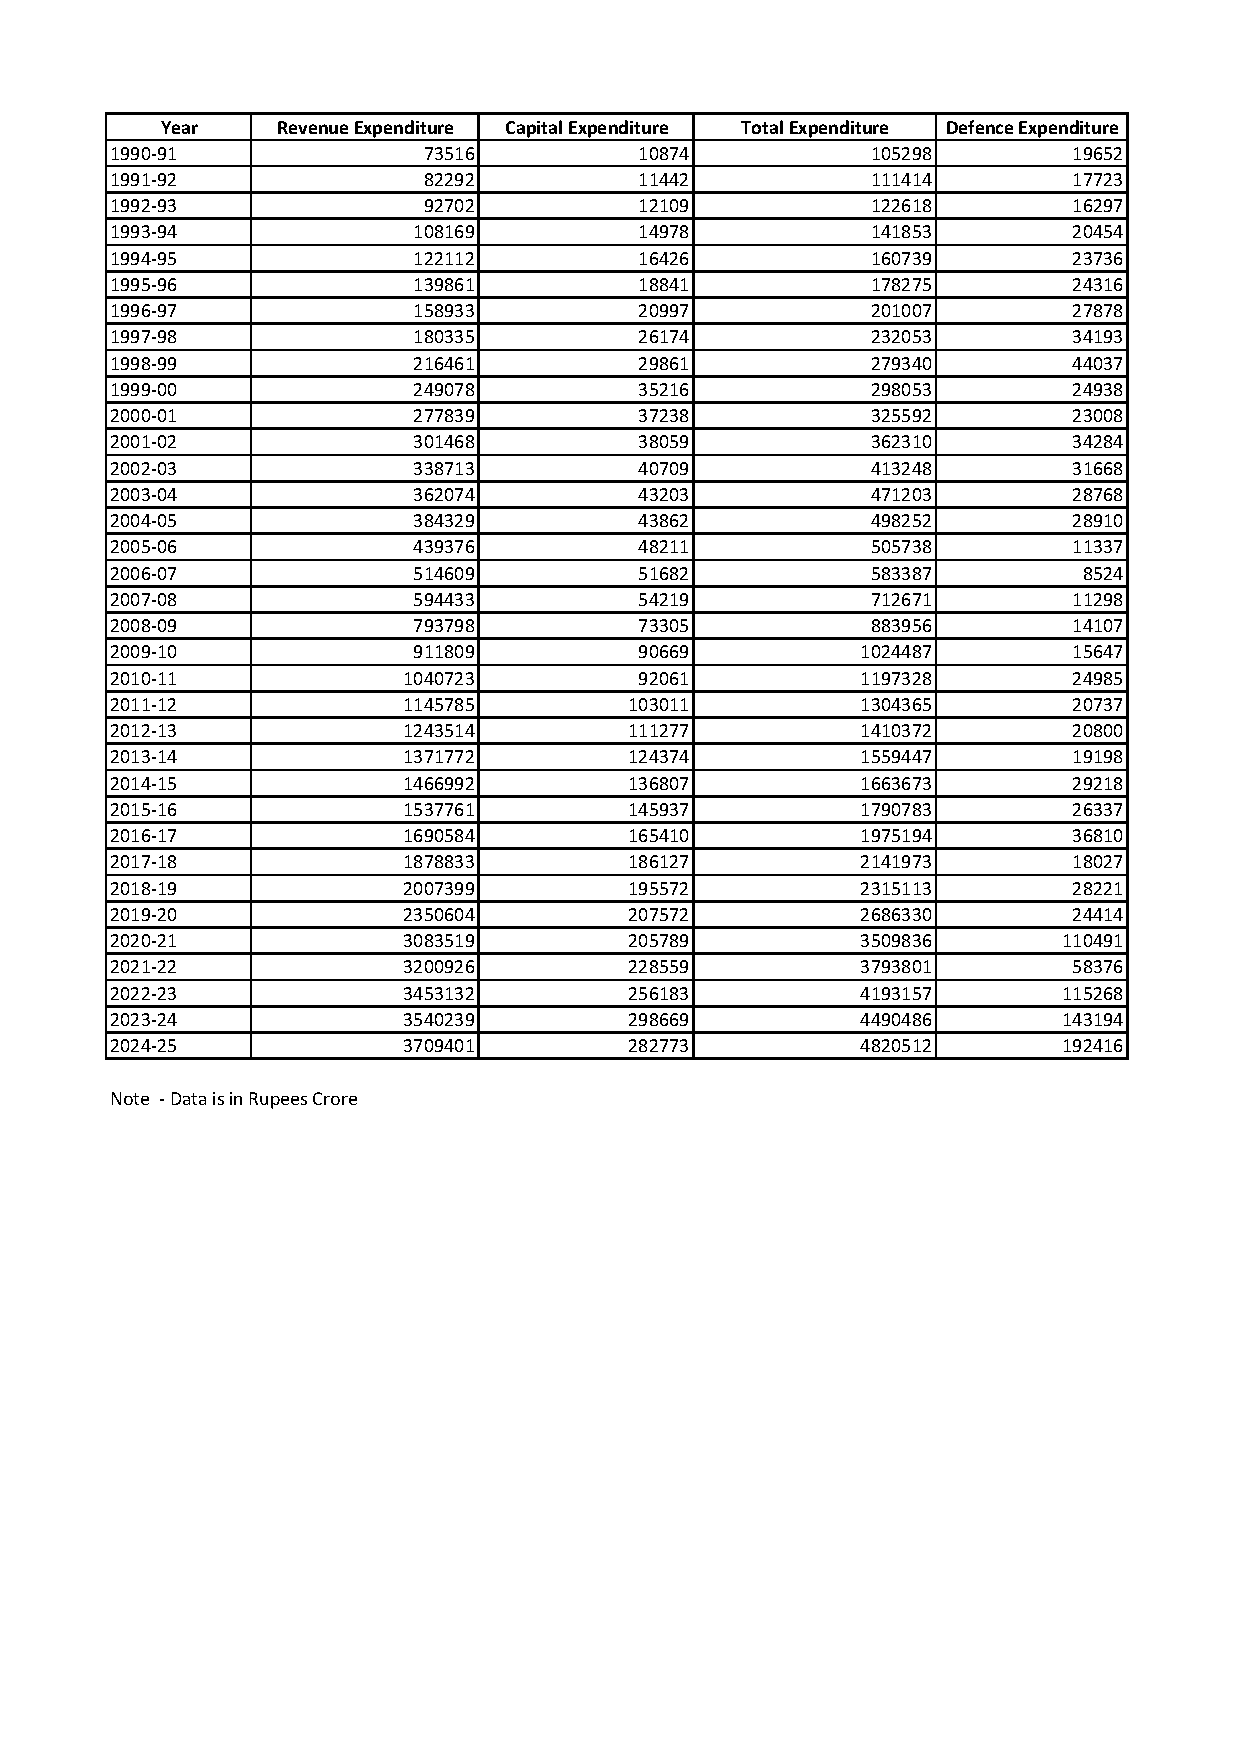
\includepdf[pages=-]{Data Assignment Q7.pdf}


\bibliographystyle{unsrt} % or another style like unsrt, apalike, etc.
\bibliography{references}

\printindex % Print the index

\end{document}
